\documentclass[aspectratio=169, 10pt, handout]{beamer}

% Slide colors
\definecolor{tx_sl_color}{RGB}{0, 0, 0}
\definecolor{bg_sl_color}{RGB}{255, 255, 255}
%\definecolor{fg_sl_color}{HTML}{B10B25}
\definecolor{fg_sl_color}{HTML}{0F6E91}

\colorlet{ft_color}{fg_sl_color!75!tx_sl_color}

\colorlet{fg_bib_color}{tx_sl_color}
\colorlet{fg_bib_color}{tx_sl_color}
\colorlet{hl_bib_color}{fg_sl_color}

% Color box colors
\definecolor{bg_cb_color}{RGB}{255, 255, 255}
\colorlet{fg_cb_color}{fg_sl_color}

% Matlab colors
\definecolor{mycolor1}{rgb}{0.00000,0.44700,0.74100}
\definecolor{mycolor2}{rgb}{0.85000,0.32500,0.09800}
\definecolor{mycolor3}{rgb}{0.92900,0.69400,0.12500}
\definecolor{mycolor4}{rgb}{0.49400,0.18400,0.55600}
\definecolor{mycolor5}{rgb}{0.46600,0.67400,0.18800}
\definecolor{mycolor6}{rgb}{0.30100,0.74500,0.93300}
\definecolor{mycolor7}{rgb}{0.63500,0.07800,0.18400}

% Set beamer theme
\setbeamercolor{normal text}{
  fg = tx_sl_color
}
\beamertemplatenavigationsymbolsempty
\setbeamercolor{frametitle}{
  bg = bg_sl_color,
  fg = fg_sl_color
}
\setbeamerfont{frametitle}{
  family = \fontfamily{qag}\selectfont\bfseries
}
\setbeamercolor{background canvas}{
  bg = bg_sl_color
}
\setbeamercolor{structure}{
  bg = bg_sl_color,
  fg = fg_sl_color
}

\makeatletter
\setbeamerfont{footline}{
  size = \scriptsize
}
\setbeamertemplate{footline}{
  \leavevmode\centering%
  \hbox{%
  \begin{beamercolorbox}[
      wd = 0.245\paperwidth,
      ht = 2.25ex,
      dp = 1.00ex,
      left
    ]{myauthor in head/foot}%
    \textcolor{ft_color}{\insertauthor{}~(\insertinstitute{})}
  \end{beamercolorbox}%
  \begin{beamercolorbox}[
      wd = 0.50\paperwidth,
      ht = 2.25ex,
      dp = 1.00ex,
      center
    ]{myframe number in head/foot}%
    \textcolor{ft_color}{\insertshortdate{}}%
  \end{beamercolorbox}%
  \begin{beamercolorbox}[
      wd = 0.245\paperwidth,
      ht = 2.25ex,
      dp = 1.00ex,
      right
    ]{mydate in head/foot}%
    \textcolor{ft_color}{\insertframenumber{}/\inserttotalframenumber{}}%
  \end{beamercolorbox}}%
  \vskip0pt%
}
\makeatother

% Enumerate and itemize
\setbeamertemplate{enumerate items}[square]
\setbeamertemplate{itemize items}[circle]
\setbeamercovered{transparent}

% Table of contents
\setbeamertemplate{section in toc}[square]
\setbeamerfont{section in toc}{
  family = \fontfamily{qag}\selectfont\bfseries
}
\setbeamerfont{subsection in toc}{
  shape = \itshape
}
\setbeamertemplate{section in toc shaded}[default][25]
\setbeamertemplate{subsection in toc shaded}[default][25]

% Figures
\usepackage{graphicx}
\usepackage{overpic}

% Math
\usepackage{amsmath}
\usepackage{amsthm}
\usepackage{amssymb}

% Font
\usepackage[default]{gillius}
%\usepackage{sfmath}
\usepackage{sansmathaccent}
\usepackage{setspace}
\usefonttheme[onlymath]{serif}
\newcommand\msmall[1]{\mbox{\small\ensuremath{#1}}}

% TikZ/PGFplots
\usepackage{tikz}
\usetikzlibrary{patterns}
\newcommand{\trollface}{\resizebox{\fontcharht\font`X}{\fontcharwd\font`X}{%

\begin{tikzpicture}[y=0.80pt, x=0.8pt,yscale=-1, inner sep=0pt, outer sep=0pt]
\path[fill=black,even odd rule] (186.5230,42.6290) .. controls
  (181.3770,46.8210) and (177.2520,52.0360) .. (177.1840,61.3090) .. controls
  (173.4610,53.8470) and (177.9210,43.3950) .. (186.5230,42.6290) -- cycle;
\path[fill=black,even odd rule] (123.9480,53.8360) .. controls
  (131.6610,49.6690) and (133.9770,68.5560) .. (129.5520,73.4490) .. controls
  (130.1610,64.4350) and (129.6880,56.5020) .. (123.9480,53.8360) -- cycle;
\path[fill=black,even odd rule] (258.4390,84.6570) .. controls
  (251.9670,92.1160) and (243.0990,85.7280) .. (234.1560,84.6570) .. controls
  (214.8650,82.3460) and (196.3430,90.9360) .. (182.7880,96.7990) .. controls
  (152.3050,81.2930) and (190.8780,59.8650) .. (221.0810,61.3090) .. controls
  (241.5710,62.2870) and (255.3680,71.4410) .. (258.4390,84.6570) --
  cycle(206.1380,68.7800) .. controls (196.6960,73.9690) and (181.3370,73.2430)
  .. (180.9200,87.4590) .. controls (194.1550,88.2420) and (196.7990,78.4330) ..
  (209.8730,79.0540) .. controls (208.5950,75.6620) and (209.3090,70.2780) ..
  (206.1380,68.7800) -- cycle(249.1000,80.9220) .. controls (248.1190,76.6100)
  and (244.5910,74.8460) .. (238.8270,75.3180) .. controls (238.2690,81.1680)
  and (246.1370,78.5920) .. (249.1000,80.9220) -- cycle;
\path[fill=black,even odd rule] (135.1560,84.6570) .. controls
  (139.6320,83.6130) and (143.7260,82.0440) .. (147.2980,84.6570) .. controls
  (147.0140,91.5340) and (139.4010,91.0810) .. (135.1560,93.9970) .. controls
  (135.1560,99.9120) and (135.1560,105.8270) .. (135.1560,111.7420) .. controls
  (129.8970,116.4450) and (122.1800,118.6910) .. (118.3440,124.8180) .. controls
  (121.4790,132.8890) and (127.0330,138.5440) .. (134.2210,142.5630) .. controls
  (138.8510,142.3020) and (140.5480,137.0180) .. (145.4290,139.7610) .. controls
  (138.6120,162.3790) and (120.0140,140.4880) .. (112.7400,131.3550) .. controls
  (110.2100,132.5610) and (109.4200,135.5060) .. (105.2680,135.0910) .. controls
  (105.7160,132.1530) and (103.9380,131.4400) .. (103.4000,129.4870) .. controls
  (96.0960,131.2120) and (93.0790,137.2230) .. (83.7870,136.9590) .. controls
  (100.7200,129.2980) and (112.9440,116.9280) .. (127.6830,107.0720) .. controls
  (127.6830,102.7140) and (127.6830,98.3550) .. (127.6830,93.9970) .. controls
  (115.4770,85.0330) and (89.1830,90.1570) .. (75.3810,82.7890) .. controls
  (83.6980,60.8440) and (125.4950,70.6300) .. (135.1560,84.6570) --
  cycle(88.4580,79.0540) .. controls (93.0320,80.8510) and (100.4610,79.8720) ..
  (104.3350,78.1190) .. controls (99.7600,76.3220) and (92.3310,77.3020) ..
  (88.4580,79.0540) -- cycle;
\path[fill=black,even odd rule] (262.1750,78.1190) .. controls
  (266.1280,76.3740) and (271.8460,80.8820) .. (278.0530,79.9870) .. controls
  (278.0700,84.9570) and (269.8980,85.7630) .. (265.9110,83.7230) .. controls
  (266.0380,81.0470) and (272.3220,84.5300) .. (272.4490,81.8550) .. controls
  (269.2020,80.4330) and (264.6140,80.3510) .. (262.1750,78.1190) -- cycle;
\path[fill=black,even odd rule] (71.6460,81.8550) .. controls
  (48.4920,80.0360) and (22.9120,89.3230) .. (22.1460,111.7420) .. controls
  (22.0350,114.9910) and (22.2010,122.2410) .. (24.9480,126.6850) .. controls
  (29.3060,133.7360) and (40.2990,130.2490) .. (43.6270,139.7610) .. controls
  (26.4310,135.6320) and (18.5280,125.8960) .. (20.2780,108.9400) .. controls
  (22.7070,85.3990) and (45.7110,76.5680) .. (71.6460,81.8550) -- cycle;
\path[fill=black,even odd rule] (335.0240,98.6670) .. controls
  (328.5190,86.1820) and (314.4580,81.2520) .. (293.9290,82.7890) .. controls
  (309.8870,79.1500) and (332.2580,83.1200) .. (335.0240,98.6670) -- cycle;
\path[fill=black,even odd rule] (262.1750,87.4590) .. controls
  (263.4210,84.8030) and (266.3280,88.1800) .. (267.7790,88.3940) .. controls
  (266.4780,91.1060) and (263.1700,88.1290) .. (262.1750,87.4590) -- cycle;
\path[fill=black,even odd rule] (219.2130,88.3940) .. controls
  (228.9990,89.9850) and (233.5670,100.3980) .. (245.3640,101.4690) .. controls
  (259.7920,102.7790) and (267.3080,92.6370) .. (279.9210,89.3270) .. controls
  (314.2440,80.3190) and (342.0750,112.2860) .. (316.3460,139.7620) .. controls
  (312.1960,130.4970) and (320.4280,125.8410) .. (319.1480,114.5440) .. controls
  (317.6560,101.3880) and (305.0200,92.5910) .. (290.1950,94.9310) .. controls
  (285.2060,95.7190) and (280.8230,101.1010) .. (275.2520,103.3370) .. controls
  (255.1770,111.3950) and (219.5950,110.7840) .. (219.2130,88.3940) -- cycle;
\path[fill=black,even odd rule] (45.4950,90.2610) .. controls
  (42.3020,96.1040) and (28.5930,99.5050) .. (33.3530,116.4120) .. controls
  (28.6240,112.2490) and (33.6510,103.5000) .. (32.4190,96.7990) .. controls
  (36.9290,94.7710) and (41.1020,92.4060) .. (45.4950,90.2610) -- cycle;
\path[fill=black,even odd rule] (84.7220,108.0070) .. controls
  (88.8510,106.8440) and (89.8150,102.5150) .. (95.9300,103.3370) .. controls
  (99.8760,115.4730) and (84.1750,115.7950) .. (72.5810,115.4790) .. controls
  (71.5810,110.8750) and (69.6390,107.2120) .. (66.0430,105.2050) .. controls
  (55.3470,104.1610) and (49.0010,107.4650) .. (39.8920,108.0080) .. controls
  (44.8020,88.7320) and (76.0790,99.0260) .. (84.7220,108.0070) -- cycle;
\path[fill=black,even odd rule] (313.5430,127.6200) .. controls
  (308.5690,129.4390) and (304.6380,127.2380) .. (299.5340,126.6850) .. controls
  (296.2380,129.2760) and (293.4220,135.3040) .. (295.7980,140.6950) .. controls
  (283.8630,150.9330) and (275.9310,169.7570) .. (264.0430,182.7230) .. controls
  (234.6970,214.7360) and (183.6470,228.5980) .. (117.4100,225.6860) .. controls
  (95.9890,224.7450) and (71.0460,222.4130) .. (60.4380,211.6760) .. controls
  (43.6320,194.6670) and (42.8320,141.9400) .. (57.6360,121.0810) .. controls
  (59.0730,118.1590) and (57.2280,111.9560) .. (60.4380,110.8080) .. controls
  (67.8970,113.3780) and (63.8270,124.2490) .. (66.0420,130.4210) .. controls
  (70.6570,143.2850) and (96.3870,151.5800) .. (114.6080,153.7710) .. controls
  (182.9370,161.9820) and (240.6520,126.1850) .. (285.5240,110.8080) .. controls
  (286.8670,107.4810) and (286.4780,102.4220) .. (289.2600,100.5350) .. controls
  (294.8400,102.4830) and (292.5530,107.1600) .. (294.8640,110.8080) .. controls
  (299.9820,118.8930) and (312.2430,119.4850) .. (313.5430,127.6200) --
  cycle(256.5710,133.2240) .. controls (256.5710,137.8940) and
  (256.5710,142.5640) .. (256.5710,147.2340) .. controls (274.1010,144.2160) and
  (289.2540,138.8220) .. (290.1940,119.2140) .. controls (274.7910,119.6880) and
  (268.9450,129.7200) .. (256.5710,133.2240) -- cycle(57.6360,143.4970) ..
  controls (59.9280,143.2360) and (61.9410,137.9240) .. (60.4380,136.9590) ..
  controls (59.6630,139.2970) and (57.8790,140.6280) .. (57.6360,143.4970) --
  cycle(205.2030,149.1020) .. controls (205.1680,155.3640) and
  (207.5990,159.1590) .. (208.0050,164.9790) .. controls (223.7610,158.0080) and
  (247.7210,159.2420) .. (249.1000,137.8940) .. controls (235.1800,138.6090) and
  (220.1700,146.3200) .. (205.2030,149.1020) -- cycle(66.9760,166.8470) ..
  controls (67.8590,159.9310) and (72.0280,150.7120) .. (67.9100,144.4320) ..
  controls (64.8520,149.0080) and (57.2650,163.7120) .. (66.9760,166.8470) --
  cycle(257.5050,174.3180) .. controls (259.8780,172.3290) and
  (263.2370,170.8490) .. (265.9110,167.7800) .. controls (269.5100,163.6490) and
  (276.6900,150.9880) .. (275.2510,150.9680) .. controls (264.4210,152.7880) and
  (248.8670,162.0370) .. (257.5050,174.3180) -- cycle(77.2500,170.5820) ..
  controls (81.8400,169.1510) and (85.3880,173.5910) .. (87.5240,171.5170) ..
  controls (84.1720,165.9570) and (90.7970,162.3580) .. (90.3260,156.5740) ..
  controls (84.8320,156.4640) and (82.4630,153.2290) .. (78.1840,151.9040) ..
  controls (73.1060,155.9740) and (76.7130,164.2210) .. (77.2500,170.5820) --
  cycle(195.8630,152.8370) .. controls (184.6230,155.6070) and
  (172.2560,157.2490) .. (161.3060,160.3090) .. controls (161.3060,164.9790) and
  (161.3060,169.6490) .. (161.3060,174.3190) .. controls (177.4140,175.4840) and
  (188.1850,171.3110) .. (200.5330,168.7150) .. controls (199.4780,162.9210) and
  (199.4950,156.0550) .. (195.8630,152.8370) -- cycle(94.0610,171.5170) ..
  controls (102.0880,173.7640) and (111.3050,174.8210) .. (122.0800,174.3190) ..
  controls (121.4640,169.8440) and (123.0400,164.0500) .. (122.0800,162.1770) ..
  controls (113.6500,161.2670) and (103.9510,161.6260) .. (97.7970,158.4420) ..
  controls (96.5510,162.7990) and (96.3510,168.2020) .. (94.0610,171.5170) --
  cycle(131.4200,162.1770) .. controls (131.6440,167.0710) and
  (129.1470,169.2430) .. (128.6180,173.3850) .. controls (135.5560,175.4760) and
  (146.2990,173.7610) .. (154.7690,174.3190) .. controls (154.7690,169.6490) and
  (154.7690,164.9790) .. (154.7690,160.3090) .. controls (145.9280,159.8740) and
  (140.7430,163.0940) .. (131.4200,162.1770) -- cycle(211.7410,178.0550) ..
  controls (210.4210,189.9590) and (217.7640,193.2010) .. (219.2130,202.3380) ..
  controls (232.4160,197.1720) and (241.9620,188.3510) .. (252.8360,180.8570) ..
  controls (247.5230,178.3850) and (247.9630,170.1630) .. (246.2980,164.0450) ..
  controls (236.3020,170.2380) and (224.6830,174.8070) .. (211.7410,178.0550) --
  cycle(168.7780,190.1960) .. controls (168.0510,199.3280) and
  (170.0950,205.6890) .. (169.7120,214.4780) .. controls (187.7230,215.6780) and
  (199.0090,210.1530) .. (211.7410,206.0730) .. controls (209.4850,196.8090) and
  (203.6060,191.1700) .. (203.3350,179.9220) .. controls (193.1930,184.7240) and
  (182.5080,188.9810) .. (168.7780,190.1960) -- cycle(66.0420,203.2710) ..
  controls (65.9030,195.9380) and (62.2210,192.1490) .. (58.5700,188.3280) ..
  controls (60.1730,194.1960) and (62.3150,199.5260) .. (66.0420,203.2710) --
  cycle(83.7880,211.6770) .. controls (81.6570,203.8460) and (79.4550,196.0850)
  .. (72.5800,192.9980) .. controls (72.0370,198.2100) and (75.3710,199.5460) ..
  (75.3820,204.2050) .. controls (74.8020,207.4170) and (70.3580,206.0980) ..
  (69.7780,207.0070) .. controls (73.0720,209.9390) and (78.5480,210.6890) ..
  (83.7880,211.6770) -- cycle(133.2880,195.8000) .. controls (133.3440,203.8380)
  and (136.3930,208.8840) .. (136.0900,217.2810) .. controls (144.8000,216.9630)
  and (154.9630,218.0960) .. (162.2410,216.3460) .. controls (161.9570,212.0840)
  and (160.6930,201.2210) .. (161.3070,192.9970) .. controls (152.8320,194.8520)
  and (141.9890,197.0030) .. (133.2880,195.8000) -- cycle(92.1930,212.6110) ..
  controls (95.7960,213.9890) and (99.2500,215.5160) .. (104.3350,215.4130) ..
  controls (103.0850,209.1910) and (98.9260,205.8780) .. (98.7310,198.6010) ..
  controls (93.8100,198.5410) and (91.8760,195.4940) .. (86.5890,195.7990) ..
  controls (87.4560,202.1920) and (94.9240,205.5740) .. (92.1930,212.6110) --
  cycle(106.2030,197.6680) .. controls (107.8940,204.6930) and
  (112.1030,209.2020) .. (113.6750,216.3470) .. controls (118.0900,216.6280) and
  (125.5740,218.7360) .. (129.5520,216.3470) .. controls (128.6800,203.5710) and
  (121.5510,192.9510) .. (106.2030,197.6680) -- cycle;
\path[fill=black,even odd rule] (197.7310,121.0820) .. controls
  (198.7120,132.7370) and (196.2330,144.5570) .. (184.6560,140.6950) .. controls
  (183.4110,132.5700) and (193.0760,132.9910) .. (191.1930,126.6850) .. controls
  (189.4350,120.7980) and (181.5510,124.0340) .. (174.3820,121.0810) .. controls
  (176.0420,109.8510) and (193.8450,115.8040) .. (197.7310,121.0820) -- cycle;
\path[fill=black,even odd rule] (200.5330,115.4790) .. controls
  (204.4700,115.3180) and (201.1740,117.5700) .. (200.5330,118.2810) .. controls
  (203.9060,128.7760) and (224.3770,116.4100) .. (228.5530,125.7530) .. controls
  (220.2110,119.9870) and (196.2170,130.8070) .. (200.5330,115.4790) -- cycle;
\path[fill=black,even odd rule] (31.4850,117.3460) .. controls
  (35.1880,120.4920) and (37.8990,124.6310) .. (42.6930,126.6860) .. controls
  (37.0450,129.1980) and (31.9330,123.1410) .. (31.4850,117.3460) -- cycle;
\path[fill=black,even odd rule] (180.9200,129.4870) .. controls
  (180.7300,132.4100) and (181.5500,136.3430) .. (179.9860,137.8930) .. controls
  (174.0290,133.1600) and (163.2140,138.0600) .. (154.7690,135.0910) .. controls
  (155.7830,124.9850) and (172.8760,127.2090) .. (180.9200,129.4870) -- cycle;
\path[fill=black,even odd rule] (258.4390,207.0070) .. controls
  (259.6460,209.1990) and (251.8250,210.0340) .. (248.1660,211.6770) .. controls
  (221.0230,223.8620) and (191.6300,245.8770) .. (151.0330,242.4980) .. controls
  (197.2180,241.0510) and (221.2870,217.4870) .. (258.4390,207.0070) -- cycle;
\path[fill=black,even odd rule] (65.1080,225.6870) .. controls
  (74.4620,238.4370) and (92.9790,242.0240) .. (113.6740,243.4320) .. controls
  (93.8120,244.9240) and (68.5880,243.6900) .. (65.1080,225.6870) -- cycle;
\path[fill=black,even odd rule] (161.3070,232.2250) .. controls
  (147.9730,232.8420) and (127.4930,235.8070) .. (112.7410,233.1590) .. controls
  (113.5640,233.3060) and (107.4200,234.1800) .. (110.8730,232.2250) .. controls
  (128.2930,233.0280) and (146.3320,230.9210) .. (161.3070,232.2250) -- cycle;
\path[fill=black,even odd rule] (127.6840,243.4320) .. controls
  (131.1270,241.2720) and (138.5660,243.1070) .. (143.5610,242.4980) .. controls
  (140.1180,244.6580) and (132.6790,242.8230) .. (127.6840,243.4320) -- cycle;
\path[fill=black,even odd rule] (38.0230,42.6290) .. controls (82.5390,0.2510)
  and (168.4500,6.1510) .. (250.9680,7.1380) .. controls (258.8160,7.2320) and
  (267.6870,5.7700) .. (274.3170,7.1380) .. controls (286.1880,9.5890) and
  (299.5410,24.1610) .. (306.0720,35.1580) .. controls (310.9170,43.3120) and
  (313.1390,55.1730) .. (317.2800,62.2430) .. controls (330.3650,84.5890) and
  (363.7570,90.1510) .. (354.6380,129.4880) .. controls (350.3990,147.7790) and
  (330.9450,155.1810) .. (321.0150,173.3850) .. controls (317.4380,179.9440) and
  (316.7720,187.3410) .. (313.5430,192.9980) .. controls (301.1180,214.7730) and
  (268.7750,231.0160) .. (241.6280,243.4320) .. controls (220.9940,252.8700) and
  (198.3130,267.1020) .. (179.0520,272.3850) .. controls (166.3570,275.8670) and
  (147.5010,278.7970) .. (128.6170,282.6580) .. controls (101.5110,288.2020) and
  (70.6950,290.9440) .. (49.2300,281.7240) .. controls (38.0840,276.9370) and
  (25.4570,265.4370) .. (23.0790,254.6390) .. controls (17.5010,229.3100) and
  (34.1810,186.6860) .. (26.8150,156.5730) .. controls (21.7590,135.9030) and
  (3.9090,121.6480) .. (10.0030,95.8650) .. controls (15.1720,74.0010) and
  (40.4630,75.0640) .. (38.0230,42.6290) -- cycle(346.2320,130.4220) .. controls
  (356.6420,101.6040) and (332.1320,76.8320) .. (298.5990,78.1190) .. controls
  (304.7890,76.0110) and (311.4390,78.0850) .. (318.2120,78.1190) .. controls
  (301.9840,58.2020) and (298.0540,17.1590) .. (264.0420,13.6760) .. controls
  (216.9920,8.8570) and (155.8050,15.1380) .. (110.8720,19.2800) .. controls
  (142.1830,27.4840) and (175.9850,13.4080) .. (208.9390,16.4780) .. controls
  (239.3500,19.3120) and (260.6870,37.8100) .. (277.1190,51.9690) .. controls
  (257.8750,41.2170) and (237.7900,21.1210) .. (208.0050,18.3460) .. controls
  (183.2390,16.0380) and (165.7270,22.7740) .. (144.4950,23.9500) .. controls
  (127.4810,24.8920) and (109.8000,20.5540) .. (94.9950,22.0820) .. controls
  (77.6030,23.8780) and (47.9860,38.7270) .. (43.6270,51.9700) .. controls
  (42.0390,56.7930) and (43.7690,62.7160) .. (41.7590,67.8470) .. controls
  (34.6190,86.0780) and (9.3930,91.1260) .. (18.4100,122.0170) .. controls
  (20.9200,130.6170) and (27.7020,135.5720) .. (30.5520,141.6310) .. controls
  (38.9450,159.4780) and (35.5640,188.2320) .. (33.3540,209.8110) .. controls
  (31.9730,223.2950) and (27.9960,238.8790) .. (30.5520,251.8390) .. controls
  (37.3950,286.5250) and (104.0000,281.3020) .. (136.0910,273.3200) .. controls
  (147.5600,270.4660) and (157.6800,265.1130) .. (166.9120,263.9800) .. controls
  (170.9690,263.4820) and (175.3540,265.1670) .. (181.8560,263.9800) .. controls
  (191.0090,262.3080) and (203.8080,252.5830) .. (214.5440,247.1680) .. controls
  (246.4100,231.0990) and (289.5540,216.8260) .. (307.0070,189.2620) .. controls
  (311.4680,182.2160) and (313.1470,170.7890) .. (316.3470,164.9790) .. controls
  (318.5940,160.8990) and (324.7580,160.0830) .. (323.8190,154.7060) .. controls
  (324.2180,156.2110) and (320.3370,157.8400) .. (320.0830,155.6400) .. controls
  (331.4360,150.5690) and (342.5940,140.4950) .. (346.2320,130.4220) -- cycle;
\path[fill=black,even odd rule] (77.2500,36.0910) .. controls
  (84.6910,22.9450) and (107.2240,33.1150) .. (124.8820,33.2890) .. controls
  (150.9490,33.5470) and (176.6190,25.1470) .. (200.5330,26.7510) .. controls
  (229.3460,28.6840) and (255.4970,42.3890) .. (269.6470,59.4400) .. controls
  (251.0790,44.9400) and (224.3560,28.4240) .. (188.3910,28.6190) .. controls
  (169.3380,28.7230) and (149.8110,36.2530) .. (124.8810,35.1570) .. controls
  (106.1230,34.3320) and (89.2790,27.8450) .. (77.2500,36.0910) -- cycle;
\path[fill=black,even odd rule] (182.7880,39.8270) .. controls
  (180.4770,39.9450) and (181.2000,38.6830) .. (182.7880,38.8920) .. controls
  (214.8340,36.0440) and (246.6730,40.8290) .. (257.5050,62.2420) .. controls
  (243.3820,43.9870) and (216.2760,38.7170) .. (182.7880,39.8270) -- cycle;
\path[fill=black,even odd rule] (134.2220,48.2320) .. controls
  (116.5830,42.4210) and (80.0680,39.9560) .. (74.4480,61.3080) .. controls
  (71.7860,48.3020) and (92.6910,40.9070) .. (112.7400,41.6940) .. controls
  (120.7850,42.0110) and (131.5240,42.7730) .. (134.2220,48.2320) -- cycle;
\path[fill=black,even odd rule] (315.4110,148.1670) .. controls
  (334.4690,145.0120) and (338.3490,122.0640) .. (335.0240,99.6010) .. controls
  (340.8540,112.7940) and (335.5300,126.2080) .. (334.0900,139.7620) .. controls
  (328.2670,142.9670) and (324.5500,148.2770) .. (315.4110,148.1670) -- cycle;
\path[fill=black,even odd rule] (47.3630,228.4880) .. controls
  (49.4920,229.7830) and (47.7110,234.9890) .. (48.2970,237.8280) .. controls
  (83.8900,267.4720) and (165.4050,250.6590) .. (207.0710,236.8940) .. controls
  (232.9420,228.3470) and (255.0540,213.7040) .. (278.9860,207.0060) .. controls
  (240.0480,233.7560) and (154.7340,260.6540) .. (83.7870,255.5720) .. controls
  (67.1820,254.3840) and (43.7210,247.9240) .. (47.3630,228.4880) -- cycle;
\end{tikzpicture}}}


% SI units
\usepackage{siunitx}
\sisetup{
  retain-zero-exponent=false,
  parse-numbers=false,
  per-mode=symbol
}

% Color boxes
\usepackage[most]{tcolorbox}
\tcbuselibrary{skins}
\tcbuselibrary{listings, breakable}

% Boxed text environment
\newtcolorbox{tbbox}[1][]{
  enhanced,
  attach boxed title to top left = {
    xshift     =  4.0mm,
    yshift     = -3.0mm,
    yshifttext = -1.0mm
  },
  colback      = bg_cb_color,
  colframe     = fg_cb_color,
  colbacktitle = fg_cb_color,
  coltitle     = bg_cb_color,
  arc          = 3.0pt,
  boxrule      = 1.0pt,
  title        = {#1},
  fonttitle    = {\fontfamily{qag}\selectfont\large\bfseries},
  halign       = flush left,
  boxed title style = {
    size       = small,
    colframe   = bg_cb_color,
    arc        = 3.0pt
  }
}
\newenvironment{bbox}[1][]{\begin{tbbox}[#1]}{\end{tbbox}}

% Boxed text environment
\newenvironment{quag}[1][]{%
  \begingroup
    {\fontfamily{qag}\selectfont\Huge\color{fg_cb_color}\bfseries{#1}} \\[1.0em]
  \endgroup
  \begingroup
}{
  \endgroup
}

% Section without toc entry
\RequirePackage{ifthen}
\newboolean{sectiontoc}
\setboolean{sectiontoc}{true} % default to true
\newcommand{\toclesssection}[1]{ % section without toc entry
  \setboolean{sectiontoc}{false}
  \section{#1}
  \setboolean{sectiontoc}{true}
}

% Table of contents at the beginning of each section
\AtBeginSection[]{
  \begin{frame}{Outline}
  \ifthenelse{\boolean{sectiontoc}}{
    \tableofcontents[
      current,
      sectionstyle=show/shaded,
      subsectionstyle=show/show/hide,
      subsubsectionstyle=show/show/show/hide
    ]
  }{
    \tableofcontents[
      current,
      sectionstyle=show/show,
      subsectionstyle=show/show/hide,
      subsubsectionstyle=show/show/show/hide
    ]
  }
  \end{frame}
}

% Add logo to the title page
\addtobeamertemplate{frametitle}{}{%
  \begin{tikzpicture}[remember picture, overlay]
    \node[anchor=north east, xshift=5pt, yshift=5pt] at (current page.north east) {\colorbox{fg_sl_color}{
\includegraphics[height=1.0cm]{logo.png}}};
    %\draw[thick, fg_sl_color] ([yshift=-1cm-6pt] current page.north west) -- ([yshift=-1cm-6pt, xshift=\paperwidth] current page.north west);
  \end{tikzpicture}%
}

% Highlighted text
\newcommand{\hi}[1]{\textcolor{fg_sl_color}{\selectfont\color{fg_cb_color}\bfseries{#1}}}
\newcommand{\hic}[1]{\begin{center}\hi{\Large{#1}}\end{center}}

% Bibliography
\PassOptionsToPackage{%
  backend      = biber,        % instead of bibtex
  bibencoding  = utf8,         % special characters
  language     = auto,         % get the language of the main document
  style        = numeric-comp, % numeric citation style
  sorting      = none,         % sorted by appearance
  maxbibnames  = 10,           % default: 3, et al.
  maxcitenames = 10,           % default: 1, et al.
  natbib       = true,         % natbib compatibility mode (\citep and \citet still work)
}{biblatex}
\usepackage{biblatex} % to display bibliography
\usepackage{bibentry} % to insert bibliography entries inline
\emergencystretch = 1.0em

\setbeamercolor{bibliography entry author}{
  bg = bg_sl_color,
  fg = fg_sl_color
}
\setbeamercolor{bibliography entry location}{
  bg = bg_sl_color,
  fg = fg_bib_color
}
\setbeamercolor{bibliography entry note}{
  bg = bg_sl_color,
  fg = fg_bib_color
}
\setbeamercolor{bibliography entry title}{
  bg = bg_sl_color,
  fg = hl_bib_color
}
\setbeamertemplate{bibliography item}[triangle]
\setbeamercolor{bibliography item}{
  bg = bg_sl_color,
  fg = fg_sl_color
}

\DeclareFieldFormat{issn}{%
  \textsc{ISSN}\addcolon\space#1
}

\DeclareFieldFormat{doi}{%
  \textsc{DOI}\addcolon\space%
  \ifhyperref{%
  \href{https://doi.org/#1}{%
    \nolinkurl{#1}%
  }
  }{%
    \nolinkurl{#1}%
  }
}

\renewcommand*{\mkbibnamefamily}[1]{% mkbibcompletename
  \ifitemannotation{jointfirst}%
    {#1\textsuperscript{\dag}}%
    {#1}
}

\addbibresource{bibliography.bib}

% Miscellanea
\usepackage{authoraftertitle}
\usepackage{hyperref}
\usepackage{chemarrow}
\usepackage[normalem]{ulem}

% Graphics path
\graphicspath{{figures}}

% Acronyms
\usepackage{acronym}
\newacro{DSM}{Direct Stiffness Method}
\newacro{FE}{Finite Element}
\newacro{RT}{Real-Time}
\newacro{FEA}{Finite Element Analysis}
\newacro{FEM}{Finite Element Method}
\newacro{LEM}{Large Expression Management}
\newacro{FFLU}{Fraction-Free Lower-Upper}
\newacro{LU}{Lower-Upper}
\newacro{MB}{Multi-Body}
\newacro{SVD}{Singular Value Decomposition}
\newacro{ODE}{Ordinary Differential Equation}
\newacro{DAE}{Differential-Algebraic Equation}
\newacro{DE}{Discrete Element}
\newacro{CAS}{Computer Algebra System}
\newacro{TPPC}{Trajectory Prescribed Path Control}
\newacro{MBD}{Multi-Body Dynamics}

% Software programs
\newcommand{\MacOS}{\textsc{MacOS}\textsuperscript{\textregistered}}
\newcommand{\Windows}{\textsc{Windows}\textsuperscript{\textregistered}}
\newcommand{\Linux}{\textsc{Linux}\textsuperscript{\textregistered}}
\newcommand{\MapleSoft}{\textsc{MapleSoft}\textsuperscript{\textregistered}}
\newcommand{\Maple}{\textsc{Maple}\textsuperscript{\textregistered}}
\newcommand{\Wolfram}{\textsc{Wolfram}}
\newcommand{\Mathematica}{\textsc{Mathematica}\textsuperscript{\textregistered}}
\newcommand{\Matlab}{\textsc{Matlab}\textsuperscript{\textregistered}}
\newcommand{\Modelica}{\textsc{Modelica}}
\newcommand{\OpenModelica}{\textsc{OpenModelica}}
\newcommand{\ModelingToolkit}{\textsc{ModelingToolkit}}
\newcommand{\Simulink}{\textsc{Simulink}\textsuperscript{\textregistered}}
\newcommand{\Mex}{\textsc{Mex}}
\newcommand{\SFunction}{\textsc{S-Function}}
\newcommand{\SymPy}{\textsc{SymPy}}
\newcommand{\Axiom}{\textsc{Axiom}}
\newcommand{\Derive}{\textsc{Derive}}
\newcommand{\Macsyma}{\textsc{Macsyma}}
\newcommand{\MuPAD}{\textsc{MuPAD}}
\newcommand{\Reduce}{\textsc{Reduce}}
\newcommand{\TrussMe}{\textsc{TrussMe-Fem}}
\newcommand{\Ansys}{\textsc{Ansys}\textsuperscript{\textregistered}}

% General commands
\newcommand{\eg}{\emph{e.g.}}
\newcommand{\ie}{\emph{i.e.}}
\newcommand{\USI}[1]{\unit{#1}}
\newcommand{\SSI}[2]{\SI{#1}{#2}}
\newcommand{\RSI}[3]{\lbrack\num{#1}{,}\ \num{#2}\rbrack\,\USI{#3}}

% Matrices and vectors
\newcommand{\dif}[2]{\ensuremath{{#1}_{#2}}}
\newcommand{\jac}[2]{\ensuremath{{#1}_{#2}}}
\newcommand{\hes}[2]{\ensuremath{{#1}_{#2}}}
\newcommand{\m}[1]{\ensuremath{\mathbf{#1}}}
\newcommand{\mx}{\ensuremath{\m{x}}}
\newcommand{\mxp}{\ensuremath{\mx^\prime}}
\newcommand{\mE}{\ensuremath{\m{E}(\mx, t)}}
\newcommand{\mg}{\ensuremath{\m{g}(\mx, t)}}
\newcommand{\ma}{\ensuremath{\m{a}(\mx, t)}}
\newcommand{\mA}{\ensuremath{\m{A}(\mx, t)}}
\newcommand{\mN}{\ensuremath{\m{N}(\mx, t)}}
\newcommand{\mK}{\ensuremath{\m{K}(\mx, t)}}
\newcommand{\mI}{\ensuremath{\m{I}}}
\newcommand{\mP}{\ensuremath{\m{P}}}
\newcommand{\mQ}{\ensuremath{\m{Q}}}
\newcommand{\mL}{\ensuremath{\m{L}(\mx, t)}}
\newcommand{\mU}{\ensuremath{\m{U}(\mx, t)}}
\newcommand{\mM}{\ensuremath{\m{M}(\mx, t)}}
\newcommand{\mb}{\ensuremath{\m{b}(\mx, t)}}
\newcommand{\mAd}{\ensuremath{\m{E}_{\m{a}}(\mx, t)}}
\newcommand{\mgd}{\ensuremath{\m{g}_{\m{a}}(\mx, t)}}
\newcommand{\mF}{\ensuremath{\m{F}(\mx, \mxp, t)}}
\newcommand{\mh}{\ensuremath{\m{h}(\mx, t)}}

\newcommand{\mv}{\ensuremath{\m{v}(\mx, t)}}
\newcommand{\mEv}{\ensuremath{\m{E}(\mx, \m{v}, t)}}
\newcommand{\mgv}{\ensuremath{\m{g}(\mx, \m{v}, t)}}
\newcommand{\mav}{\ensuremath{\m{a}(\mx, \m{v}, t)}}
\newcommand{\mvv}{\ensuremath{\m{v}(\mx, \m{v}, t)}}
\newcommand{\mAv}{\ensuremath{\m{A}(\mx, \m{v}, t)}}
\newcommand{\mNv}{\ensuremath{\m{N}(\mx, \m{v}, t)}}
\newcommand{\mKv}{\ensuremath{\m{K}(\mx, \m{v}, t)}}
\newcommand{\mLv}{\ensuremath{\m{L}(\mx, \m{v}, t)}}
\newcommand{\mUv}{\ensuremath{\m{U}(\mx, \m{v}, t)}}
\newcommand{\mMv}{\ensuremath{\m{M}(\mx, \m{v}, t)}}
\newcommand{\mbv}{\ensuremath{\m{b}(\mx, \m{v}, t)}}
\newcommand{\mAdv}{\ensuremath{\m{E}_{\m{a}}(\mx, \m{v}, t)}}
\newcommand{\mgdv}{\ensuremath{\m{g}_{\m{a}}(\mx, \m{v}, t)}}
\newcommand{\mFv}{\ensuremath{\m{F}(\mx, \mxp, \m{v}, t)}}
\newcommand{\mhv}{\ensuremath{\m{h}(\mx, \m{v}, t)}}
\newcommand{\mhiv}{\ensuremath{\m{h}_{i}(\mx, \m{v}, t)}}
\newcommand{\mhuv}{\ensuremath{\m{h}_{u}(\mx, \m{v}, t)}}

% Title page
\title{Symbolic Computation Methods for the Numerical Solution of Dynamic Systems Described by Differential-Algebraic Equations}
\author{Davide Stocco}
\institute{University of Trento}
\date{August 1, 2024}

\begin{document}

%!TEX root = main.tex

\begin{frame}[noframenumbering, plain]
  \begin{tikzpicture}[remember picture, overlay]
    \fill[fg_sl_color] (current page.south west) rectangle ([xshift = 0.25\paperwidth] current page.north west);
    \node at ([xshift = 0.125\paperwidth, yshift = -0.4\paperheight] current page.north west){
      
\includegraphics[width = 0.15\paperwidth]{logo}
    };
    \node at ([xshift = 0.125\paperwidth, yshift = -0.6\paperheight] current page.north west){
      
\includegraphics[width = 0.15\paperwidth]{unitn}
    };
  \end{tikzpicture}
  \begingroup
    \flushright
    \begin{minipage}{0.75\linewidth}%
      \flushright%
      \begin{spacing}{1.25}
        {\fontfamily{qag}\selectfont\large\bfseries\color{fg_sl_color}\MyTitle{}}%
      \end{spacing}
      \vspace{1.5em}%
      \textsc{PhD thesis presentation by} \emph{Davide Stocco} \\%
      \textsc{Supervisors}: \emph{Enrico Bertolazzi} \& \emph{Francesco Biral}%
      \vspace{1.5em} \\%
      \MyDate%
    \end{minipage}
    \par
  \endgroup
\end{frame}

% That's all Folks!
%!TEX root = main.tex

\toclesssection{Introduction and Motivation}

\begin{frame}{Introduction and Motivation}{The Simulation of Dynamic Systems}
  \begin{columns}
    \begin{column}[c]{0.6\textwidth}
      \uncover<1->{%
        \hi{\large Why do we need simulation?} \\
        It is used to \\
        \begin{itemize}\small
          \setlength{\itemsep}{0.0em}
          \item[\raisebox{-1pt}{\scalebox{0.8}{\faCogs}}] \emph{predict} the behavior
          \item[\raisebox{-1pt}{\scalebox{0.8}{\faConnectdevelop}}] \emph{design} and \emph{optimize}
          \item[\raisebox{-1pt}{\scalebox{0.8}{\faHourglassHalf}}] accelerate development and testing
          \item[\raisebox{-1pt}{\scalebox{0.8}{\faCarCrash}}] risk-free testing environment
          \item[\raisebox{-1pt}{\scalebox{0.8}{\faDollarSign}}] \emph{reduce} development costs
        \end{itemize}
      }
      \vspace{0.5em}
      \uncover<2->{%
        \hi{\large Simulations' \textbf{complexity} is increasing!} \\
        Higher \textbf{fidelity}, more \textbf{complexity}, more \dots \\
        \begin{itemize}\small
          \setlength{\itemsep}{0.0em}
          \item[\raisebox{-1pt}{\scalebox{0.8}{\faCog}}] components \\
          \item[\raisebox{-1pt}{\scalebox{0.8}{\faCompress}}] interactions \\
          \item[\raisebox{-1pt}{\scalebox{0.8}{\faDesktop}}] computational resources \\
          \item[\raisebox{-1pt}{\scalebox{0.8}{\faHourglassHalf}}] computation time
        \end{itemize}
      }
      \end{column}
    \begin{column}[c]{0.4\textwidth}
      \centering
      \visible<3->{\includegraphics[width=0.52\textwidth, trim={0cm 0cm 4.65cm 0cm}, clip]{figures/vehicle_modules.eps}}
    \end{column}
  \end{columns}
\end{frame}

\subsection{Dynamic Systems as a Collection of Subsystems}

\begin{frame}{Introduction and Motivation}{Dynamic Systems as a Collection of Subsystems}
  \begin{columns}
    \begin{column}[c]{0.6\textwidth}
      \begin{itemize}
        \item<1-> Complex systems are divided into \textbf{subsystems} \\
        \begin{small}
          \quad\, \begin{tabular}{ccc}
            \raisebox{-1pt}{\scalebox{0.8}{\textcolor{fg_sl_color}{\faCogs}}} mechanical &
            \raisebox{-1pt}{\scalebox{0.8}{\textcolor{fg_sl_color}{\faBolt}}} electrical &
            \raisebox{-1pt}{\scalebox{0.8}{\textcolor{fg_sl_color}{\faFire}}} thermal \\
            \raisebox{-1pt}{\scalebox{0.8}{\textcolor{fg_sl_color}{\faOilCan}}} hydraulic &
            \raisebox{-1pt}{\scalebox{0.8}{\textcolor{fg_sl_color}{\faWaveSquare}}} control & \dots
          \end{tabular}
        \end{small}
        \item<2-> Subsystems are modeled by \textbf{equations} \\
        \begin{small}
          \qquad \emph{algebraic} \\
          \qquad ordinary \emph{differential} \\
          \qquad \emph{differential-algebraic} \\
          \qquad other types
        \end{small}
        \item<3-> The \textbf{challenges} are \hic{\normalsize Speed \qquad Accuracy \qquad Efficiency}
      \end{itemize}
    \end{column}
    \begin{column}[c]{0.4\textwidth}
      \centering
      \only<1->{\includegraphics[width=\textwidth]{figures/vehicle_modules.eps}}
    \end{column}
  \end{columns}
\end{frame}

\subsection{Solution Approaches}

\begin{frame}{Introduction and Motivation}{Solution Approaches}
  \begin{columns}
    \begin{column}[c]{0.45\textwidth}
      The \textbf{solution} of these equations can be \\
      \begin{itemize}[<+->]
        \item \textbf{Analytical} \\
        \begin{small}
          \qquad \textcolor{mycolor2!95!black}{deep understanding of the problem} \\
          \qquad \textcolor{mycolor2!95!black}{rare and difficult to achieve} \\
          \qquad \textcolor{mycolor5!95!black}{low computational resources}
        \end{small}
        \item \textbf{Numerical} \\
        \begin{small}
          \qquad \textcolor{mycolor5!95!black}{well-established and widely used} \\
          \qquad \textcolor{mycolor3!95!black}{parametricity loss} \\
          \qquad \textcolor{mycolor2!95!black}{high computational resources}
        \end{small}
        \item \textbf{Mixed analytical/numerical} \\
        \begin{small}
          \qquad \textcolor{mycolor3!95!black}{\emph{ad hoc}, for specific cases} \\
          \qquad \textcolor{mycolor5!95!black}{balance between the two approaches} \\
          \qquad \textcolor{mycolor5!95!black}{reduced computational resources}
        \end{small}
      \end{itemize}
    \end{column}
    \begin{column}[c]{0.6\textwidth}
      \centering
      \small
      \vspace{-2.0em}
      \begin{tabular}{>{\centering\arraybackslash} m{3.75cm} >{\centering\arraybackslash} m{3.75cm}}
        \visible<3->{\vspace{-3.0em}$\msmall{\begin{array}{c}
          \text{\hi{Tire-road interaction (A1-2)}} \\[0.25em]
          \mathbf{P} = \frac{1}{V} \int\nolimits_\mathcal{V} \text{proj}(\mathbf{x}, \partial\mathcal{G}) \, \text{d}\mathcal{\mathbf{x}} \\[0.1em]
          \mathbf{\hat{n}} = \int\nolimits_\mathcal{V} \mathbf{d}(\mathbf{x},\mathbf{h}_y) \, \text{d}\mathcal{\mathbf{x}}
        \end{array}}$ &
        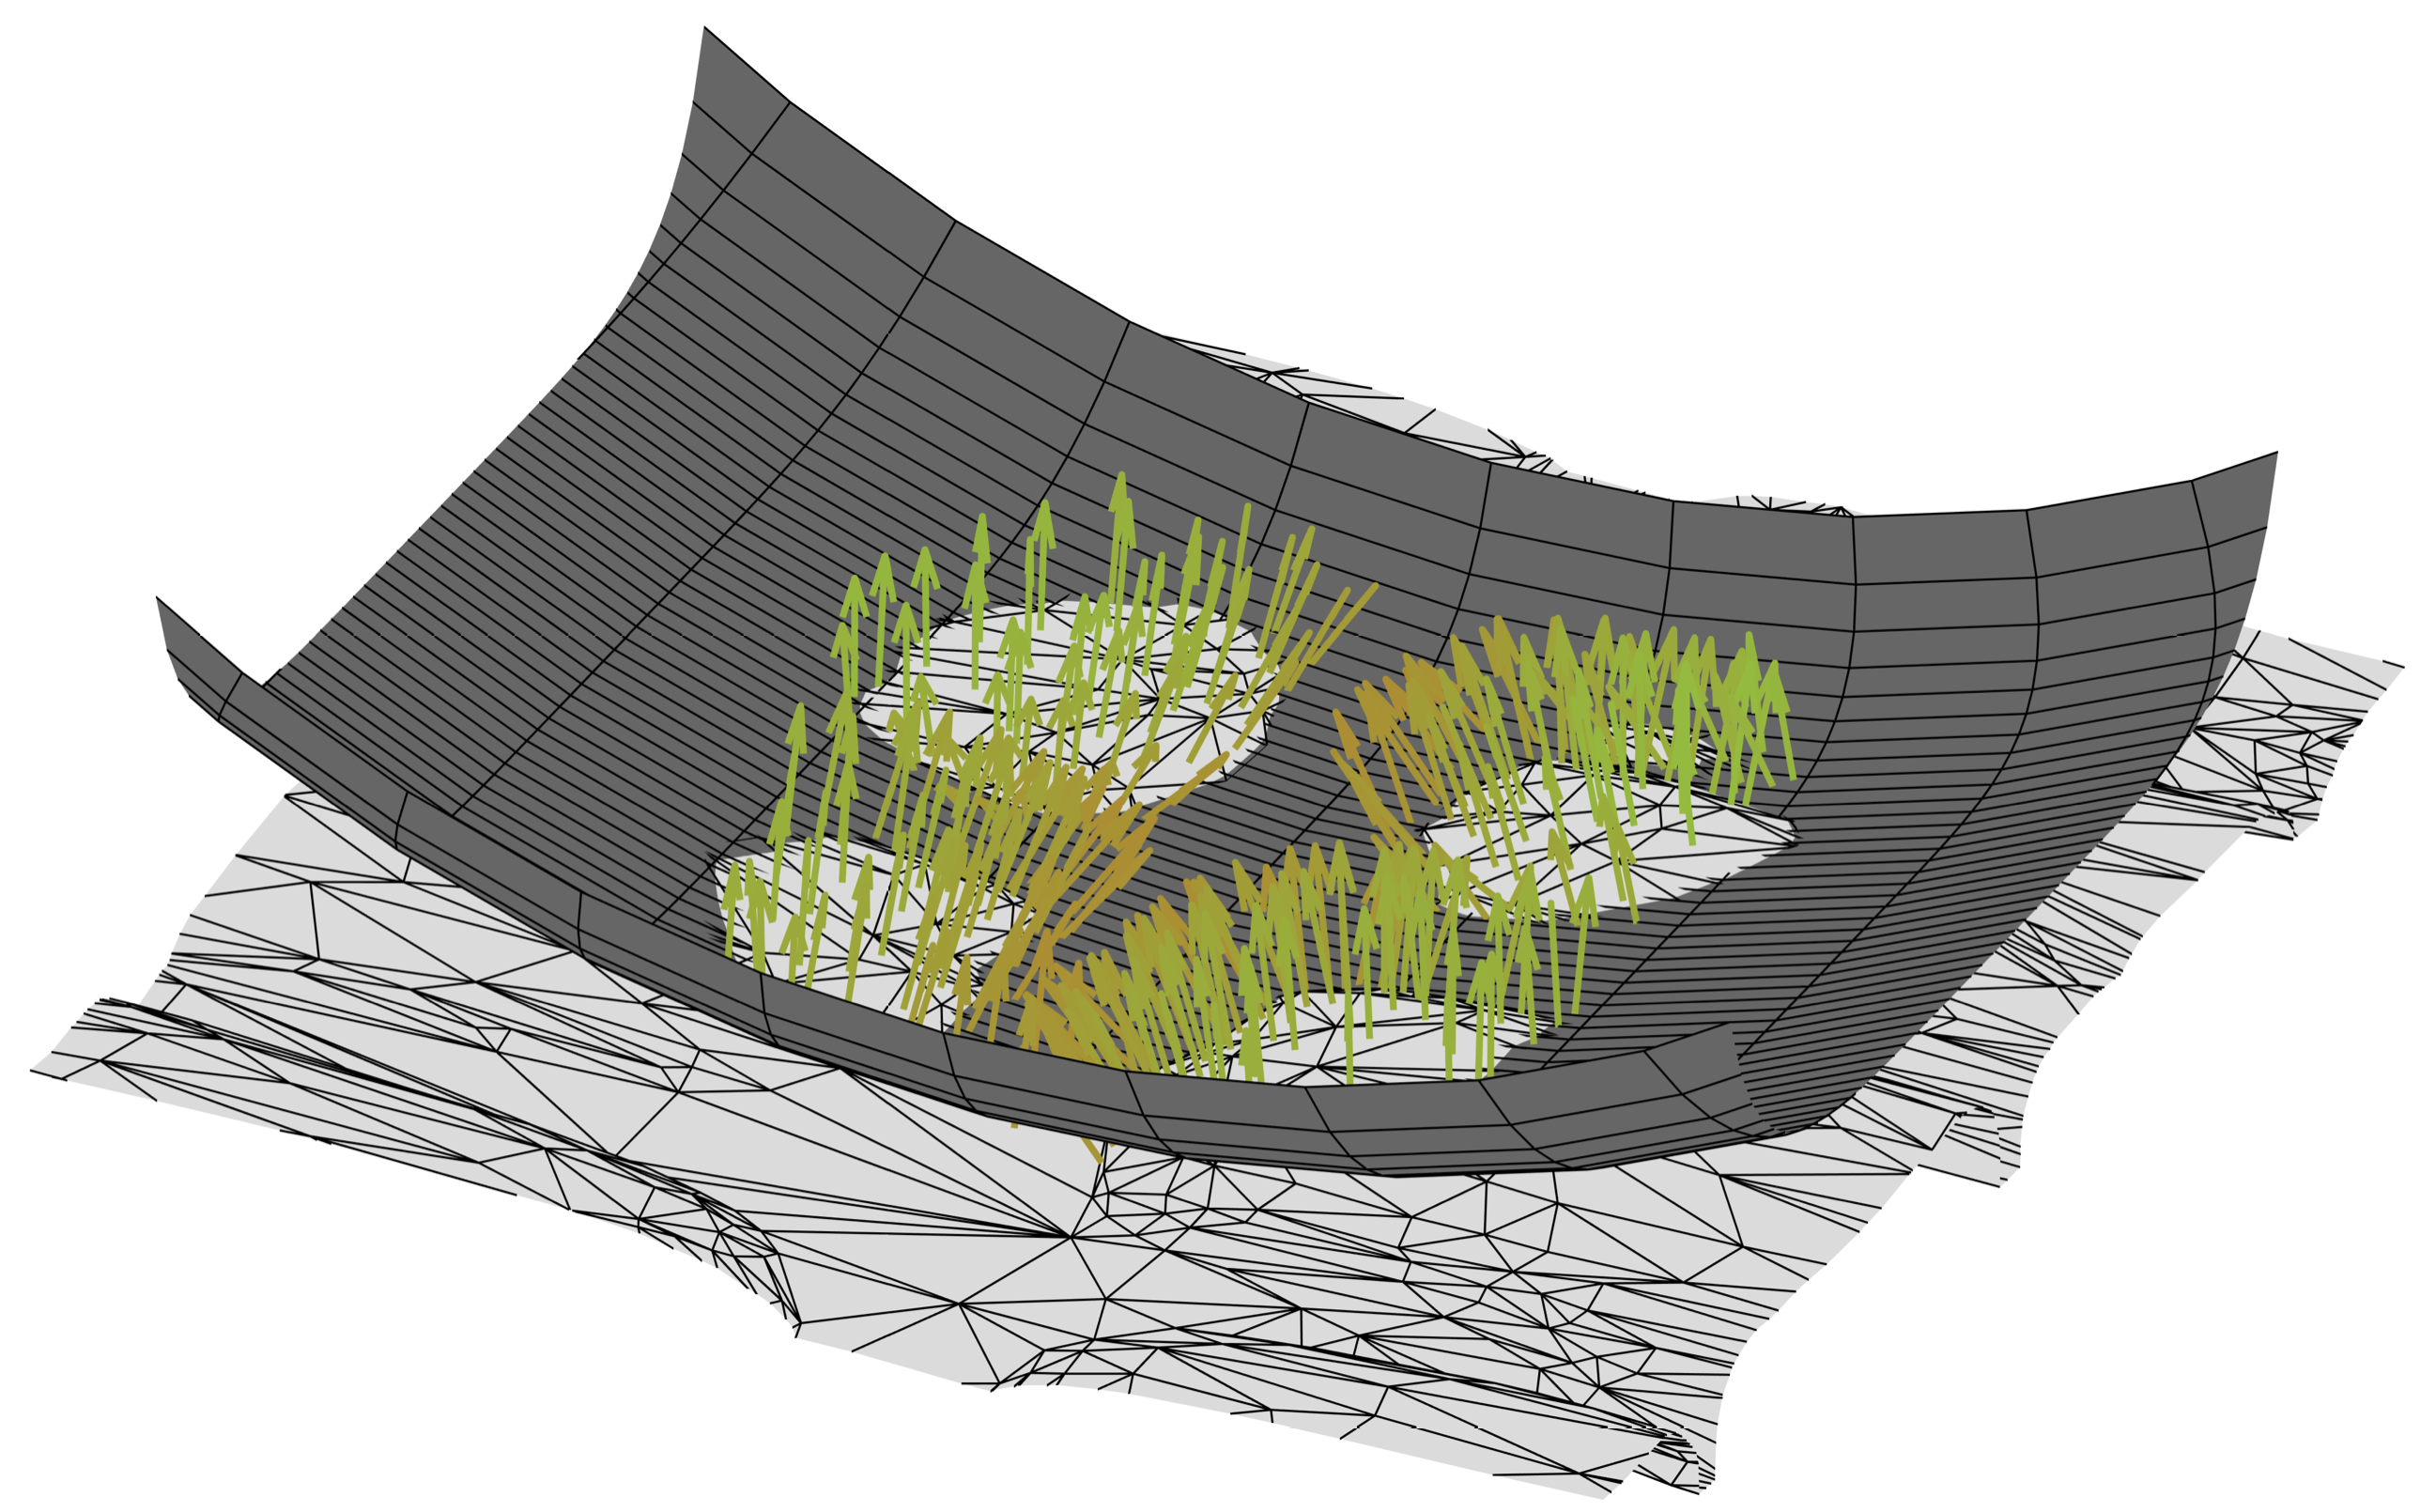
\includegraphics[width=0.4\textwidth]{figures/enve_intersection.png}} \\
        \visible<3->{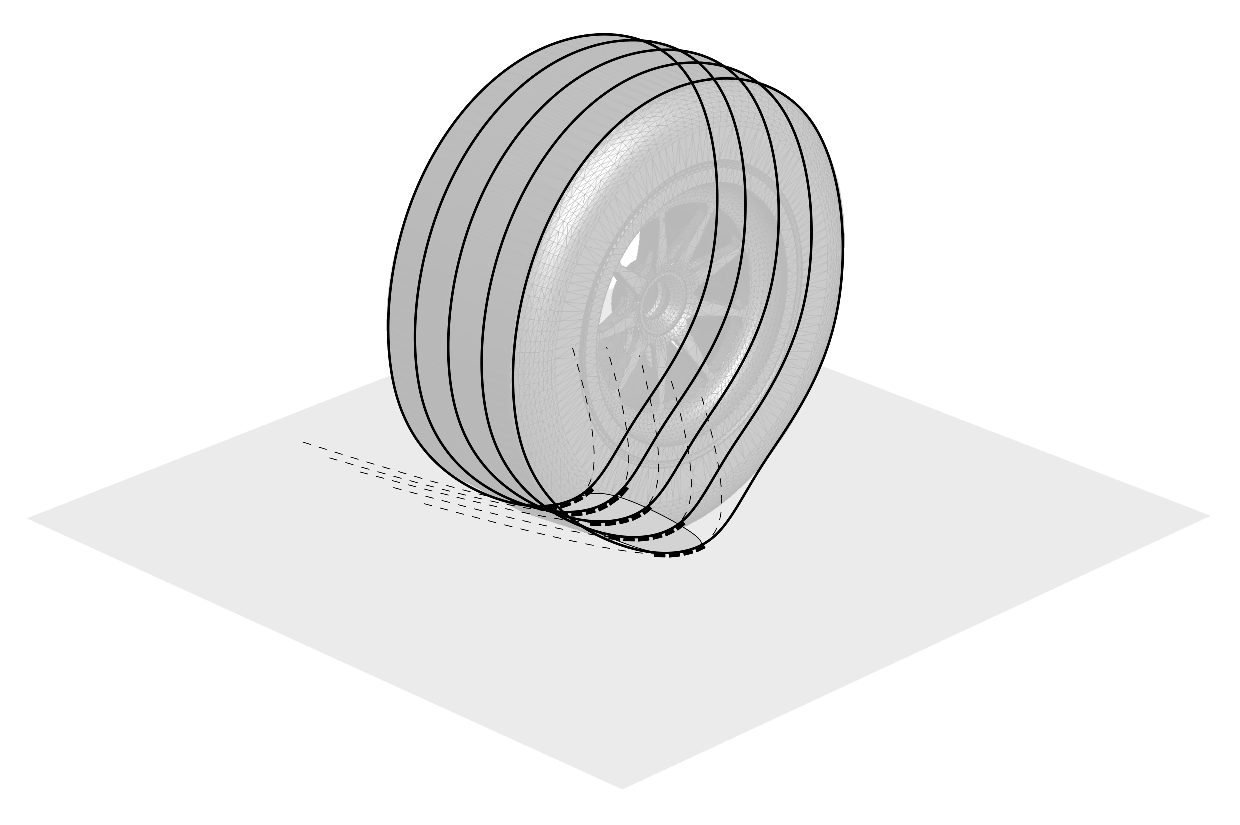
\includegraphics[
          width=0.35\textwidth, trim={4.5cm 3.5cm 4.5cm 0cm}, clip
          ]{figures/brush_model_simplified.eps} &
          \vspace{-3.0em}$\msmall{\begin{array}{c}
            \text{\hi{Tire model (A3)}} \\[0.25em]
            \mathbf{F}(F_z, \sigma_x, \sigma_y, \varphi, \gamma, p, T, t) \\[0.1em]
            \mathbf{M}(F_z, \sigma_x, \sigma_y, \varphi, \gamma, p, T, t)
          \end{array}}$} \\
          \visible<3->{\vspace{-2.0em}$\begin{array}{c}
            \text{\hi{Suspension System (A4)}} \\[0.25em]
            \text{Macro-element FE model} \\
            \text{Modified MB-DAE system}
            \end{array}$ &
          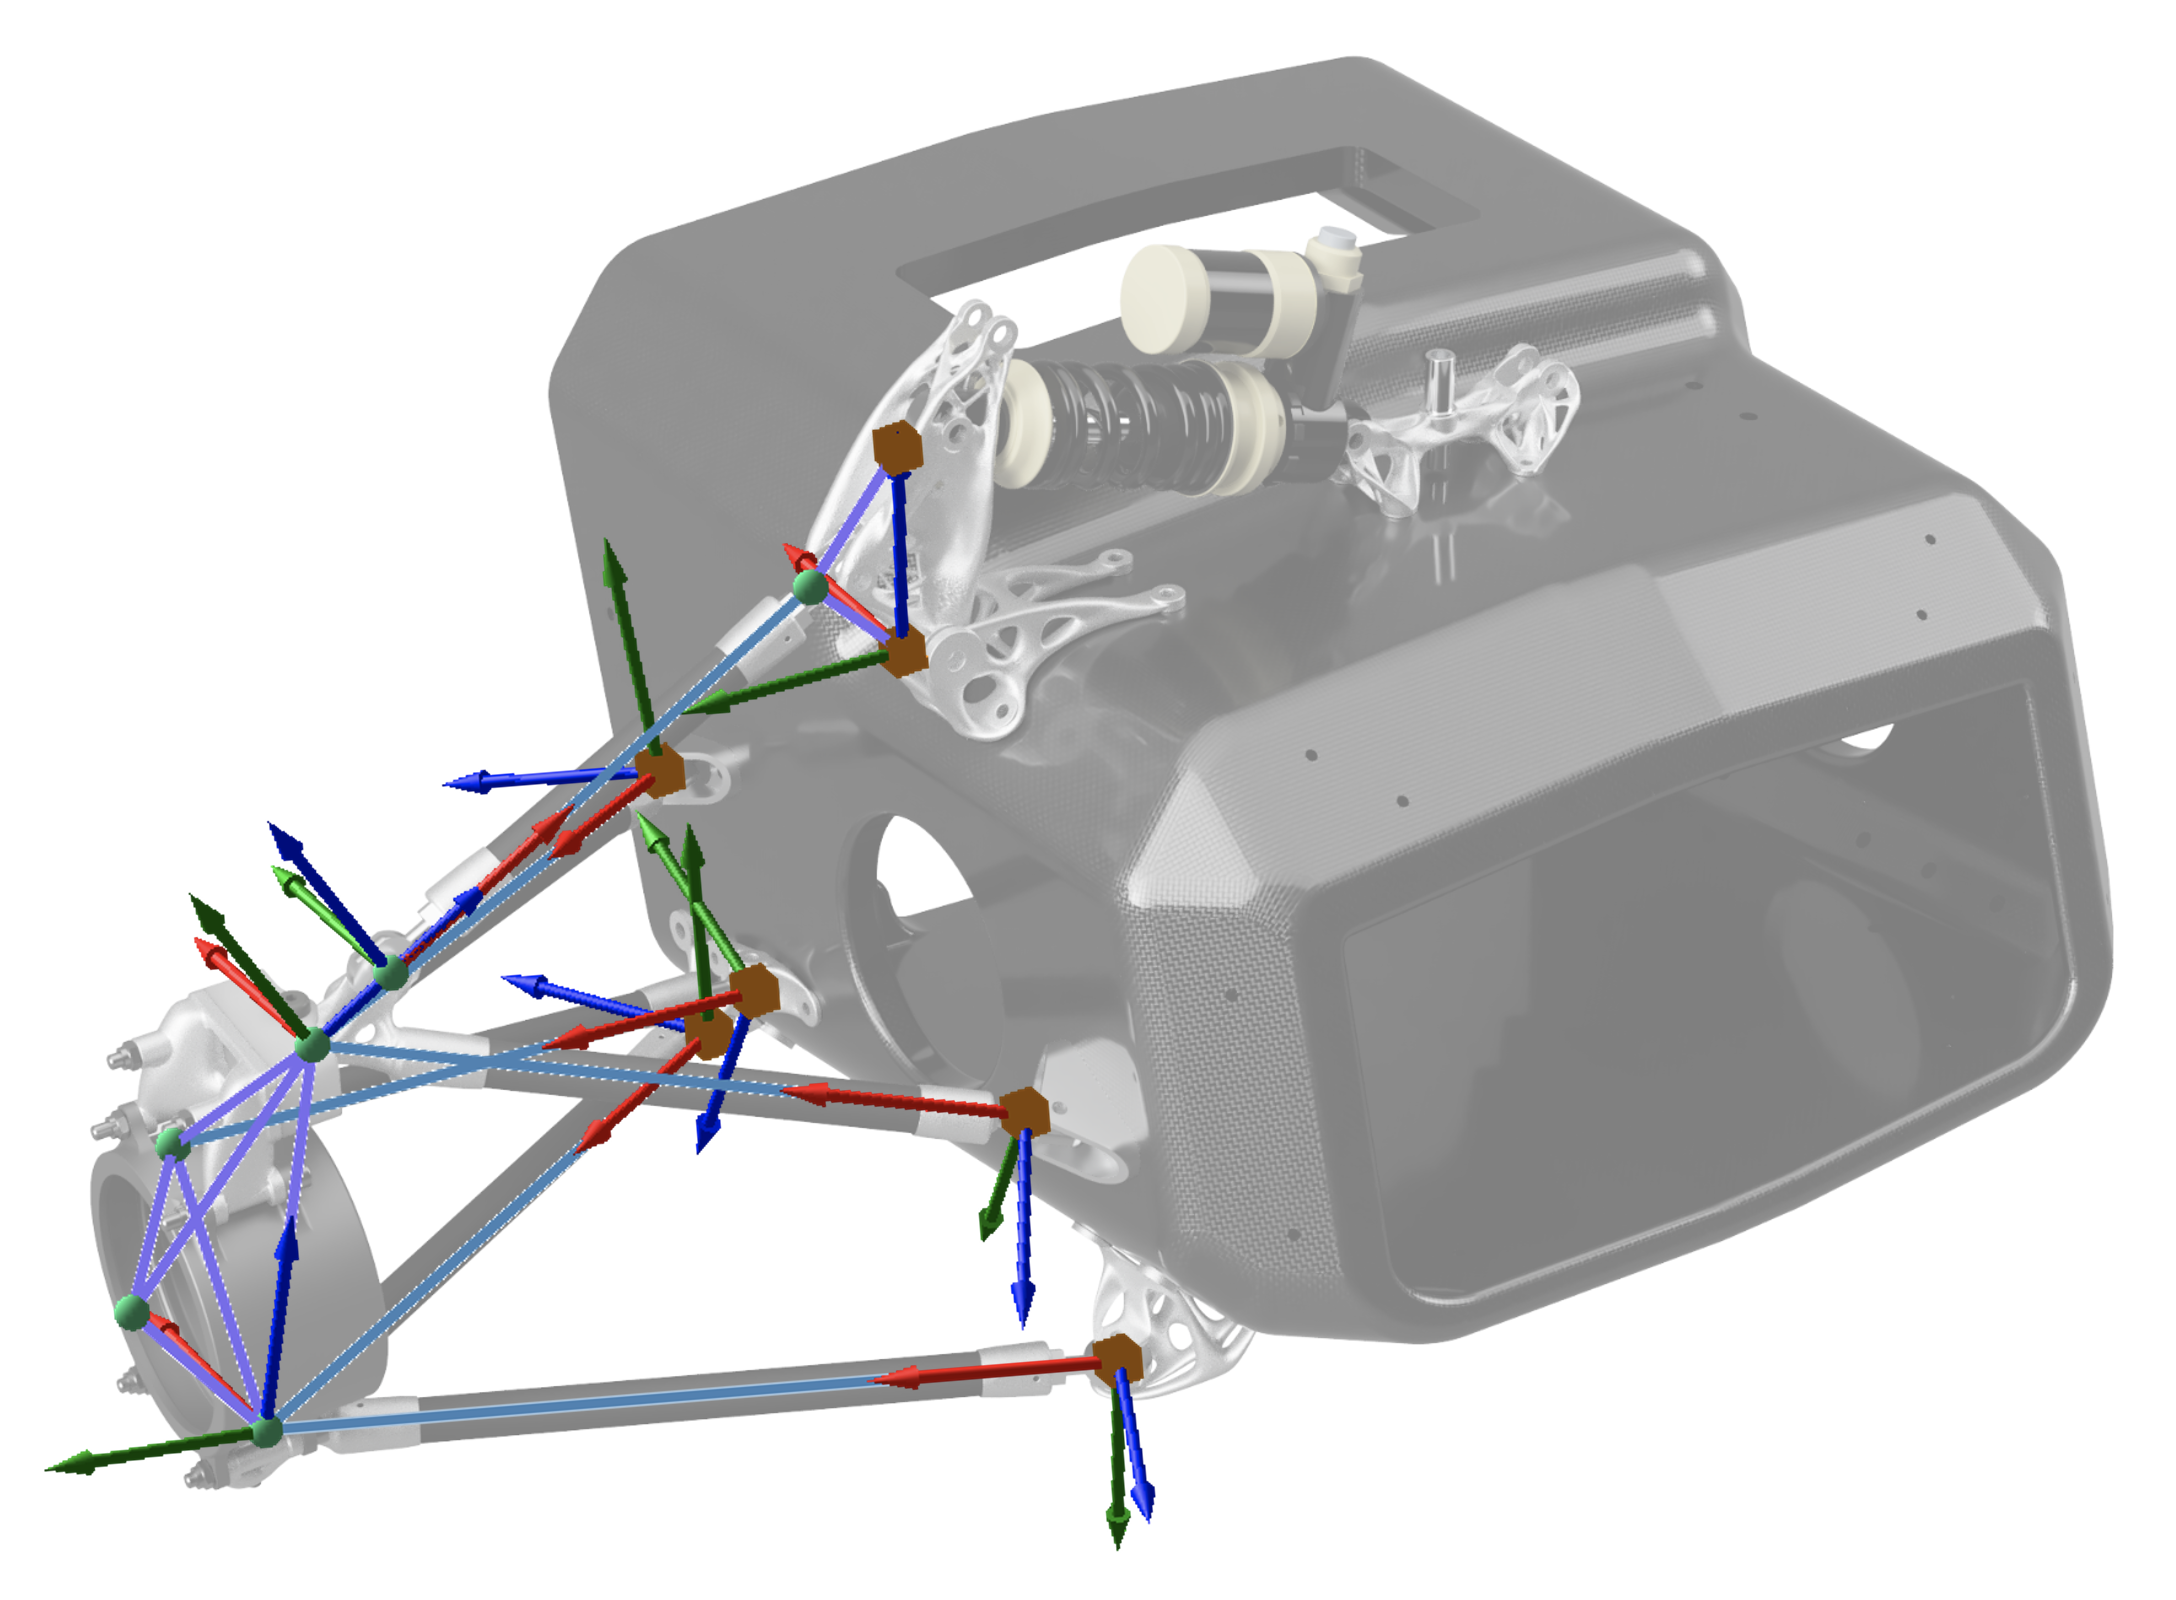
\includegraphics[width=0.4\textwidth]{figures/fade_overview.png}}
      \end{tabular}
    \end{column}
  \end{columns}
\end{frame}

\begin{frame}{Introduction and Motivation}{A Representative Example: FSAE Double Wishbone Suspension}
  \vspace{-2.0em}
  \centering{\begin{tikzpicture}[scale=0.5]
    \node at (-3,2) {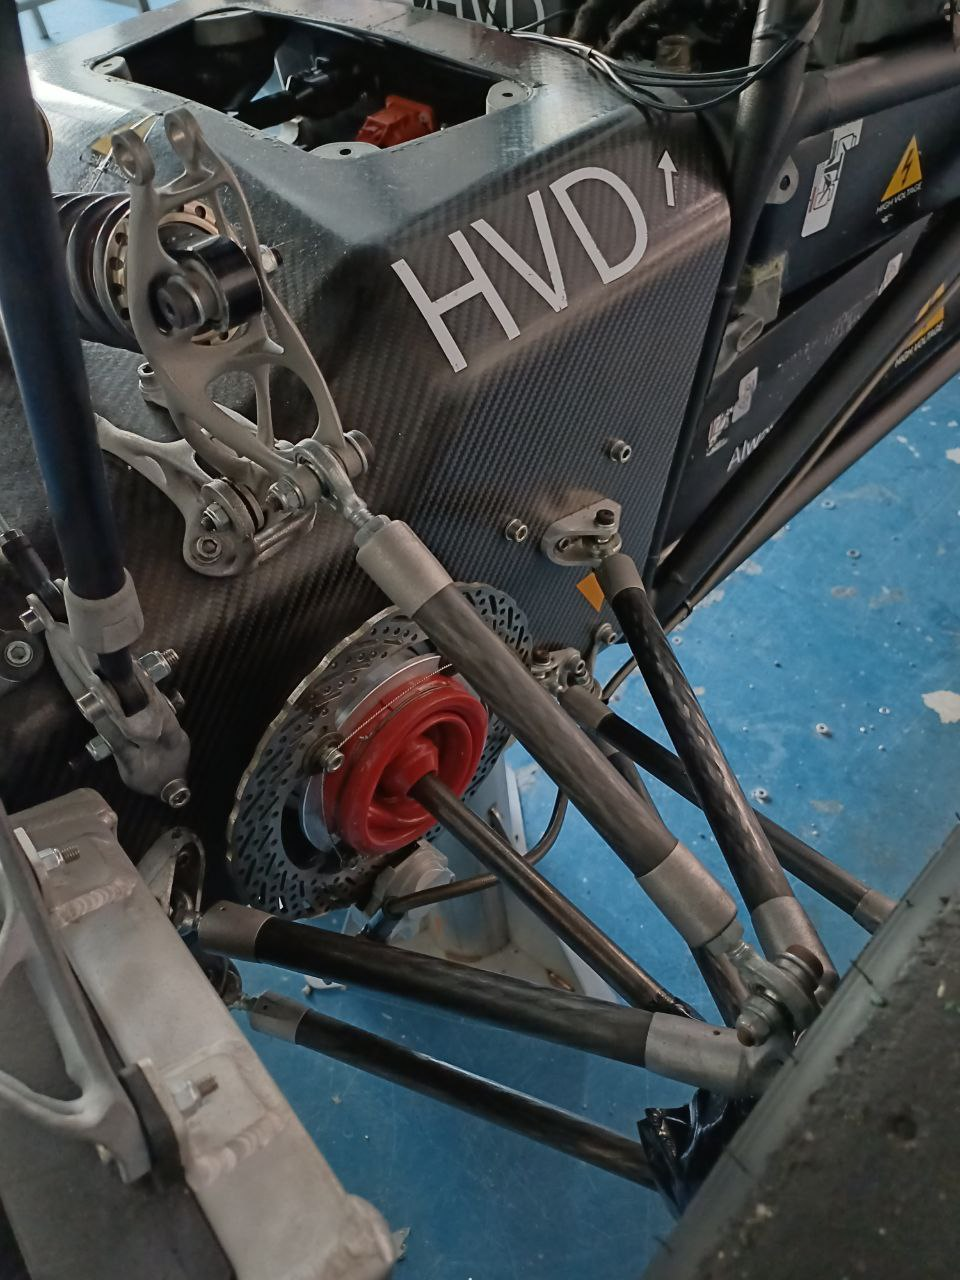
\includegraphics[width=0.125\textwidth]{figures/fsae.jpeg}};
    \node at (3,2) {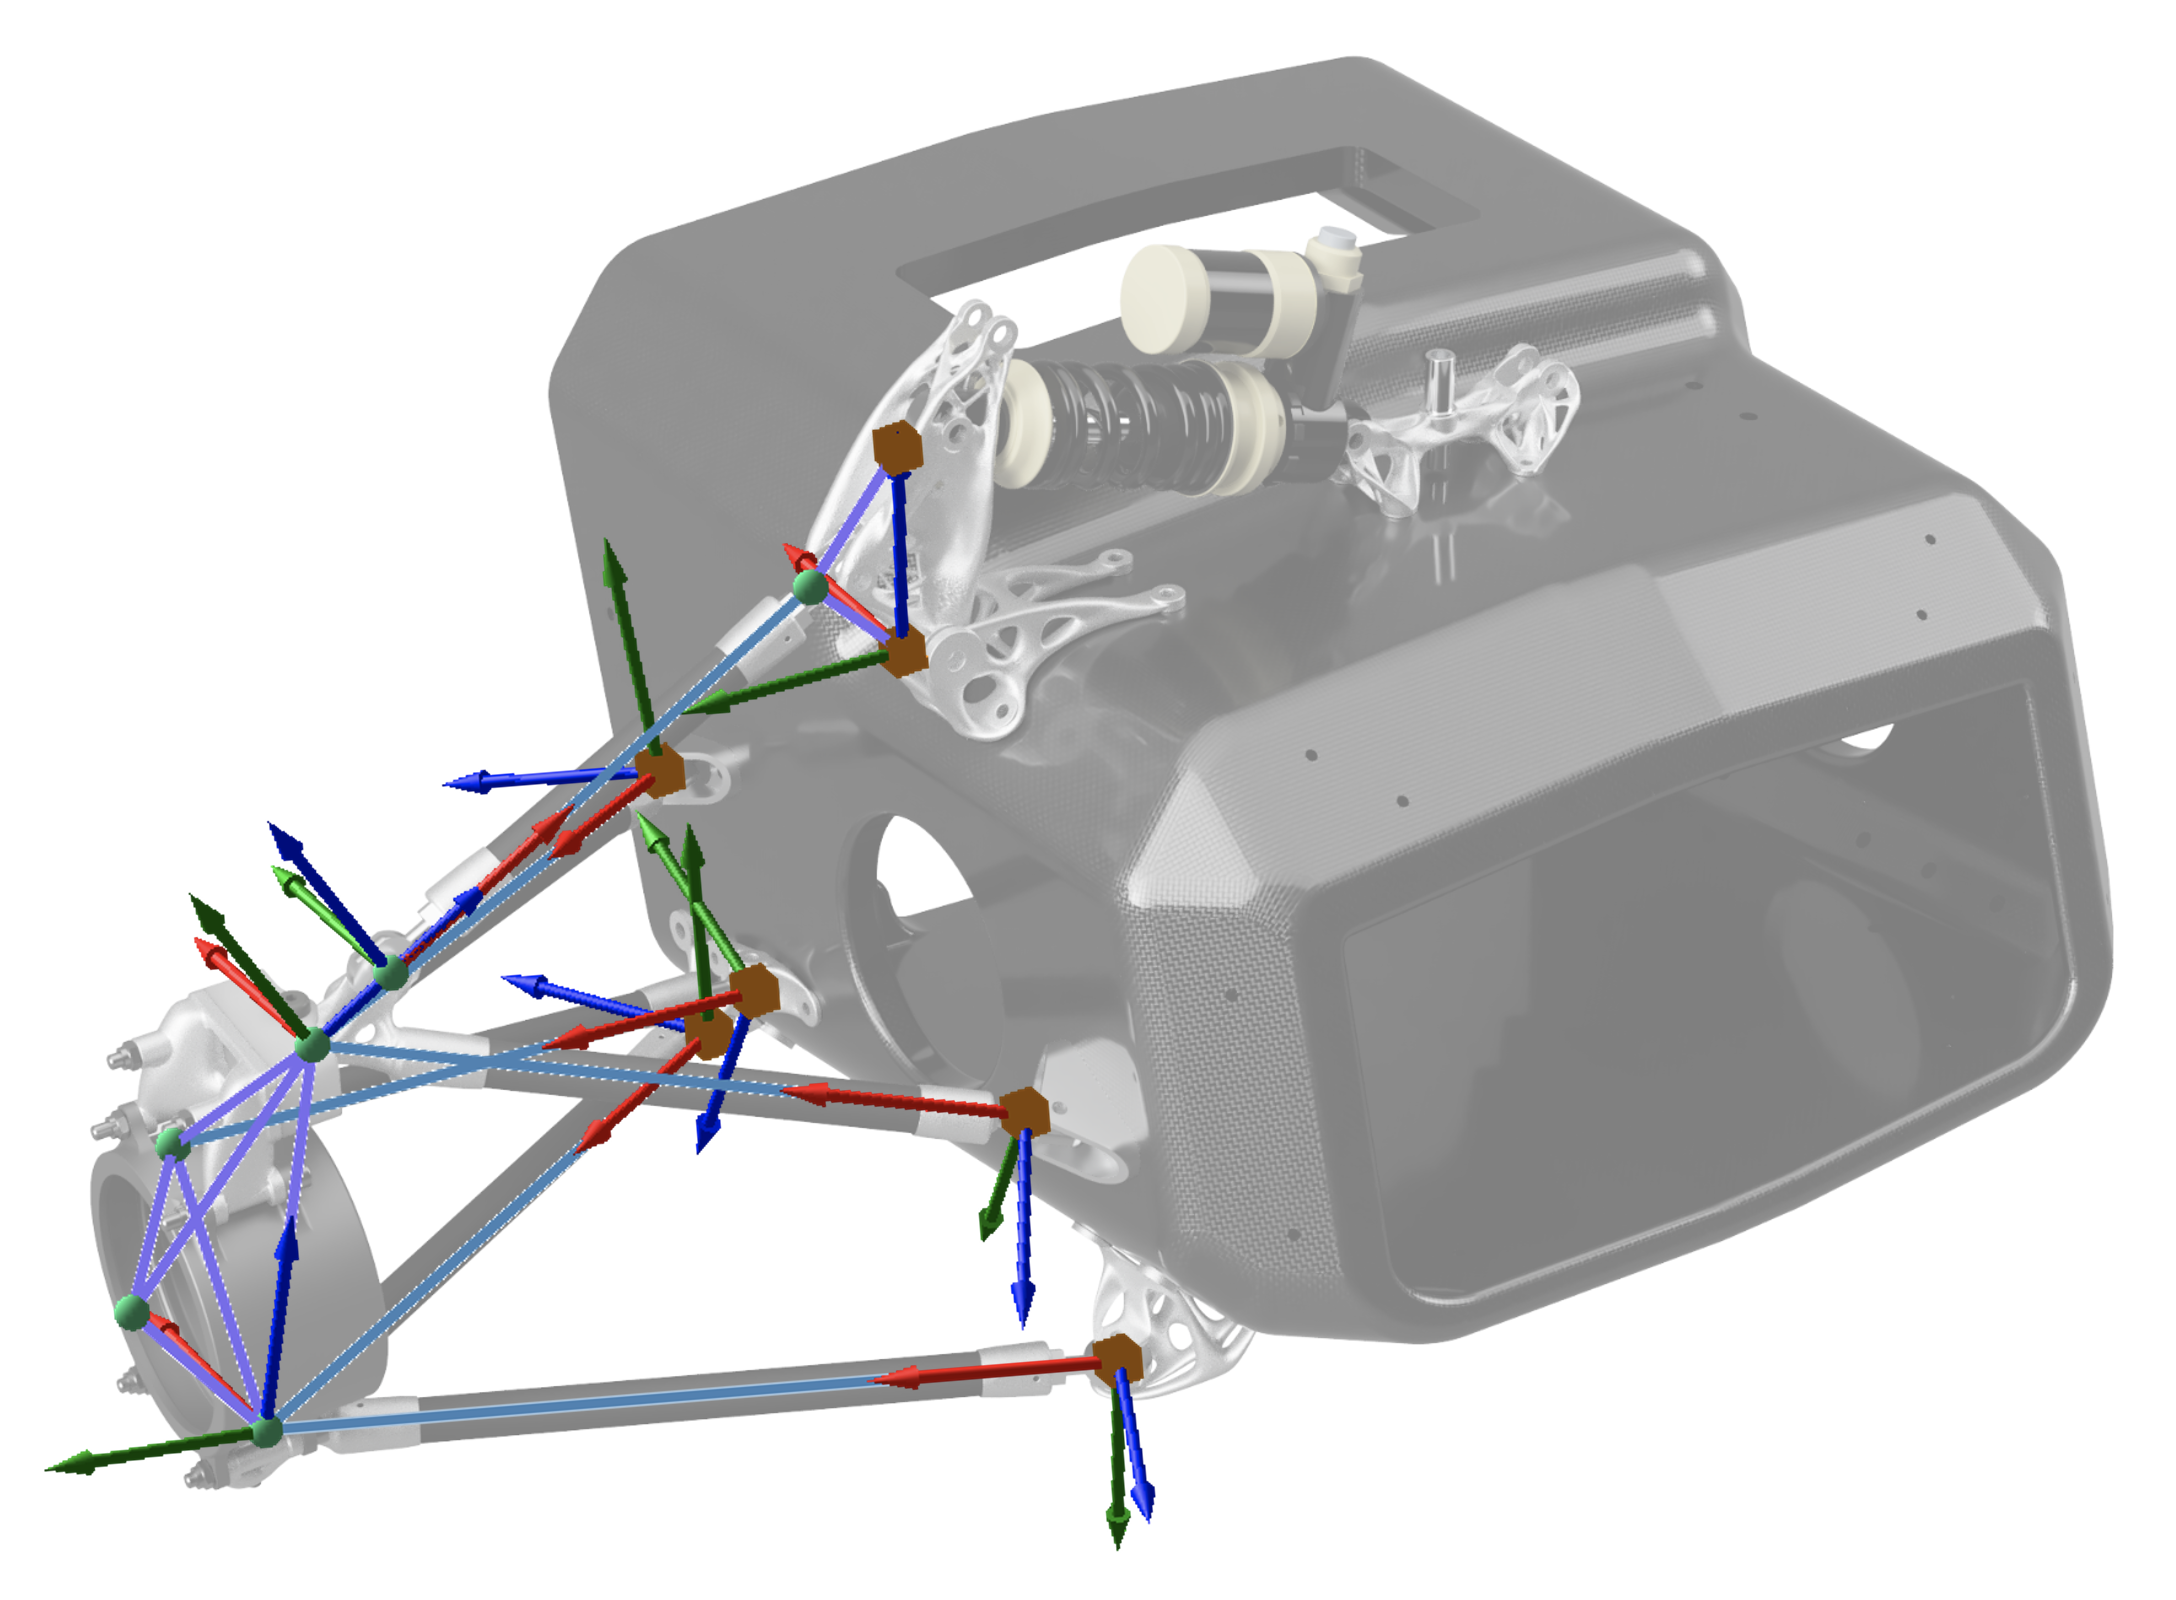
\includegraphics[width=0.25\textwidth]{figures/fade_overview.png}};
    \uncover<2->{
      \draw[fg_sl_color, thick, -stealth] (-2,-1) -- (-4.0,-3);
      \draw (-0.525\textwidth,-3.25) node[below, text width=0.5\textwidth] {
        \centering
        \hi{\large Flexibility of components} \\
        \small
        Macro-element \acs{FE} model \\[-1.5em]
        \begin{equation*}
          \begin{bmatrix}
            \mathbf{K}_{ff, 72 \times 72}(\mathbb{R}) & \mathbf{K}_{fs, 72 \times 66}(\mathbb{R}) \\
            \mathbf{K}_{sf, 66 \times 72}(\mathbb{R}) & \mathbf{K}_{ss, 66 \times 66}(\mathbb{R})
          \end{bmatrix} \begin{bmatrix}
            \mathbf{d}_{f, 72}(\mathbb{R}) \\
            \mathbf{d}_{s, 66}(\mathbb{R})
          \end{bmatrix} = \begin{bmatrix}
            \mathbf{f}_{f, 72}(\mathbb{R}) \\
            \mathbf{f}_{s, 66}(\mathbb{R})
          \end{bmatrix}
        \end{equation*}
        \vspace{-0.5em}
        \begin{equation*}
          \autorightarrow{\text{symbolic matrix}}{\text{factorization of $\mathbf{K}_{ff}$}} \quad
          \begin{aligned}
            \mathbf{d}_{f} &= \mathbf{K}_{ff}^{-1}\left(\mathbf{f}_{f} - \mathbf{K}_{fs}\mathbf{d}_{s}\right) \\
            \mathbf{f}_{s} &= \mathbf{K}_{sf}\mathbf{d}_{f} + \mathbf{K}_{ss}\mathbf{d}_{s}
          \end{aligned}
        \end{equation*}
    };}
    \uncover<3->{
      \draw[fg_sl_color, thick, -stealth] (+2,-1) -- (+4.0,-3);
      \draw (0.525\textwidth,-3.25) node[below, text width=0.5\textwidth] {
        \centering
        \hi{\large Dynamics of the system} \\
        \small
        Modified \acs{MB}-\acs{DAE} system \\[-1.5em]
        \begin{equation*}
          \msmall{\left\{\!\!\!\!\begin{array}{l}
            \mathbf{y} = \mathbf{x} + \mathbf{d} \\
            \mathbf{M}(\mathbf{y}) \ddot{\mathbf{y}} + \mathbf{r}(\mathbf{x}, \dot{\mathbf{x}}, \mathbf{d}, \dot{\mathbf{d}}) = \mathbf{f}(t) \\
            \boldsymbol{\Phi}_{\mathbf{x}}(\mathbf{x})^\top \boldsymbol{\lambda} = \mathbf{K}_c(\mathbf{x}) \mathbf{d} + \mathbf{C}_c(\mathbf{x}) \dot{\mathbf{d}} + \mathbf{b}(\mathbf{x}, \dot{\mathbf{x}}, t) \\
            \boldsymbol{\Phi}(\mathbf{x}) = \mathbf{0}
          \end{array}\!\!\!\!\right.}
        \end{equation*} \\[-0.5em]
        This problem requires more knowledge and tools!
      };}
  \end{tikzpicture}}
\end{frame}

\subsection{Dynamic Systems Described by \acsp{ODE} and \acsp{DAE}}

\begin{frame}{Introduction and Motivation}{Dynamic Systems Described by \acsp{ODE} and \acsp{DAE}}
  \begin{itemize}
    \item Let us take a step back to generic \textbf{dynamic systems}
      \vspace{0.5em}
      \setlength{\tabcolsep}{3.5em}
      \centering{\small\begin{tabular}{cc}
          \hi{\acsp{ODE}}                                               & \hi{\acsp{DAE}} \\
          \textcolor{mycolor5!95!black}{Easy to initialize}            & \textcolor{mycolor2!95!black}{Hard to initialize} \\
          \textcolor{mycolor5!95!black}{Strong theoretical foundation} & \textcolor{mycolor3!95!black}{Complex theoretical foundation} \\
          \textcolor{mycolor5!95!black}{Efficient numerical methods}   & \textcolor{mycolor3!95!black}{Require \emph{ad hoc} numerical methods} \\
          \textcolor{mycolor2!95!black}{Some models do not fit}        & \textcolor{mycolor5!95!black}{State-of-the-art in modeling} \\
      \end{tabular}}
    \vspace{0.25em}
    \raggedright
    \item \acsp{ODE} have \textbf{well-enstablished} theoretical foundation, \acsp{DAE} do not
    \item Existing tools for \acsp{DAE} are not as \textbf{mature} and \textbf{efficient} as \acsp{ODE} tools
    \item From an engineering perspective, this is a \textbf{problem} (\textcolor{fg_sl_color}{\scalebox{0.8}{\faHourglassHalf\,\faDollarSign\,\faCarCrash\,\faSadTear}})
  \end{itemize}
  \uncover<2->{
    \centering
    \vspace{0.5em}
    Therefore, the question is \\[-1.0em]
    \hic{\large How can we improve the state-of-the-art in the solution of \acsp{DAE}?}
  }
\end{frame}

% That's all Folks!

%!TEX root = main.tex

\section{\aclp{DAE}}

\begin{frame}{\aclp{DAE}}{A Brief Introduction}
  \begin{columns}
    \begin{column}{0.65\textwidth}
      \acp{DAE} are \dots
      \begin{enumerate}
        \item a generalization of \acp{ODE} \dots
        \begin{equation*}
          \begin{array}{c}
            \text{\hi{\acp{ODE}}} \\
            \mxp = \m{f}(\mx, t)
            \phantom{~}
          \end{array}
          \qquad\qquad
          \begin{array}{c}
            \text{\hi{\acp{DAE}}} \\
            \mF = \m{0}
          \end{array}
        \end{equation*}
        \dots with $\m{JF}_{\mxp}$ possibly singular. \\[1.0em]
        \item equivalent to an \ac{ODE} system with \textbf{constraints}. \\[1.0em]
        \item state-of-the-art in the modeling of dynamical systems:
        \begin{itemize}
          \item differential equations describe the system's \textbf{dynamics};
          \item algebraic equations constrain the system to a \textbf{manifold}.
        \end{itemize}
      \end{enumerate}
    \end{column}
    \begin{column}{0.35\textwidth}
      \centering
      \small
      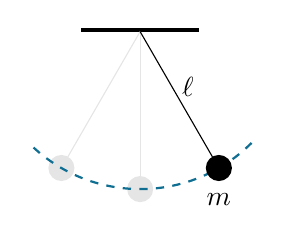
\begin{tikzpicture}[scale=0.5]
        \fill (-1.5,0) rectangle (1.5,0.1);
        \draw[tx_sl_color!10] (0,0) -- (-90:4) node [fill, circle]{};
        \draw[tx_sl_color!10] (0,0) -- (-120:4) node [fill, circle]{};
        \draw[fg_sl_color, thick, dashed] (2.8284, -2.8284) arc (-45:-135:4);
        \draw (0,0) -- (-60:4) node[fill, circle](m){};
        \node at (m) [below, yshift=-2mm] {$m$};
        \node at (1.2142, -1.4142) {$\ell$};
      \end{tikzpicture}
      \begin{equation*}
        \begin{array}{c}
          \text{\ac{ODE}} \\ \text{model}
        \end{array}
        \begin{cases}
          \theta^\prime = \omega \\
          \omega^\prime = -\dfrac{g}{\ell} \sin(\theta)
        \end{cases}
      \end{equation*}
      \begin{equation*}
        \begin{array}{c}
          \text{\ac{DAE}} \\ \text{model}
        \end{array}
        \begin{cases}
          x^\prime = u \\
          y^\prime = v \\
          u^\prime = -2x\lambda \\
          v^\prime = -2y\lambda - gm \\
          \, \textcolor{fg_sl_color}{0 = x^2 + y^2 - \ell^2}
        \end{cases}
      \end{equation*}
    \end{column}
  \end{columns}
\end{frame}

\subsection{Solution of \aclp{DAE}}

\begin{frame}{Solution of \aclp{DAE}}{\underline{\acp{DAE} are not \acp{ODE} cit. Linda Petzold}}
  \vspace{-1.5cm}\hspace{4.25cm}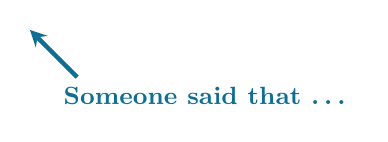
\begin{tikzpicture}[scale=0.6]
    \draw[fg_sl_color, ultra thick, -stealth] (0.0,0.0) -- (-1.0,1.0);
    \node at (2.75,0.0) [below]{\small \hi{Someone said that \dots}};
  \end{tikzpicture} \\[1.0em]

  Is the solution of \acp{DAE} a straightforward extension of \acp{ODE}?
  \begin{itemize}
    \item \textbf{No}, otherwise we would not have been here (scientifically speaking).
    \item Numerical integration of \acp{DAE} is \textbf{challenging}.
    \item A \textbf{reformulation} of the \ac{DAE} system is typically required.
  \end{itemize}
  \vspace{1.0em}
  We end up with two main approaches \dots
  \vspace{1.5em}
  \begin{columns}
    \begin{column}[t]{0.5\textwidth}
      \centering
      \hi{\large Direct Discretization}
    \end{column}
    \begin{column}[t]{0.5\textwidth}
      \centering
      \hi{\large Index Reduction}
    \end{column}
  \end{columns}
  \vspace{1.5em}
  \centering{\hi{\large \dots or a mix between the two!}}
\end{frame}

\subsubsection{Direct Discretization}

\begin{frame}{Solution of \aclp{DAE}}{Direct Discretization}
  \begin{bbox}[The Fundamental Idea]
    Approximate $\mxp$ through a \textbf{discretization formula} like a \emph{finite difference scheme} or a \emph{polynomial quadrature}, \eg{}, the Radau collocation.
  \end{bbox}
  \vspace{0.5em}
  This discretization can be written as an \textbf{implicit Runge-Kutta} method as
  \begin{equation*}
    \begin{array}{l}
      \m{F}\left(\m{x}_{k} + h_k\displaystyle\sum_{j=1}^{s}a_{ij} \m{K}_j, \m{K}_i, t_{k} + c_i h_k\right) = \m{0} \\[0.5em]
      \m{x}_{k+1} = \m{x}_{k} + h_k\displaystyle\sum_{i=1}^{s} b_i \m{K}_i
    \end{array}
    \quad \text{for} \quad
    \begin{array}{c}
      i = 1, \dots, s \\
      k = 0, 1, \dots
    \end{array}
  \end{equation*}
  If $(a_{ij})$ is non-singular (along with other conditions), we can solve for $\mxp_k = \m{K}_i$ at each step.
\end{frame}

\subsubsection{Index Reduction}

\begin{frame}{Solution of \aclp{DAE}}{The Index \dots Or better Yet, The Indices}
  The index is a ``measure of difficulty'' in the analytical or numerical treatment of the \acp{DAE} \dots
  \begin{itemize}
    \item Different approaches in classifying such difficulties led to \textbf{different index concepts}:
    \begin{columns}
      \begin{column}[t]{0.45\textwidth}
        \centering\small
        differentiation index \\
        structural index \\
        tractability index
      \end{column}
      \begin{column}[t]{0.45\textwidth}
        \centering\small
        differentiation index \\
        structural index \\
        tractability index
      \end{column}
    \end{columns}
    \item Some indices coincides under certain conditions.
    \item The old-but-gold and is the \textbf{differentiation index}, or ``the'' index.
  \end{itemize}
  \vspace{0.5em}
  \begin{bbox}[The Differentiation Index]
    It is the minimum number of differentiations required to transform a \ac{DAE} system into its underlying \ac{ODE} system.
  \end{bbox}
\end{frame}

\begin{frame}{Solution of \aclp{DAE}}{Index Reduction}
  \begin{bbox}[The Fundamental Idea]
  \vspace{-1.0em}
  \begin{equation*}
      \begin{array}{c}
        \text{High-index} \\
        \text{\ac{DAE}}
      \end{array}
      \quad \autorightarrow{\text{index}}{\text{reduction}} \quad
      \begin{array}{c}
        \text{Index-1 \ac{DAE}}  \\
        \text{or} \\
        \text{\ac{ODE}}
      \end{array} {\hspace{-0.75em}+\,\text{Invariants}}
      \quad \autorightarrow{\text{numerical}}{\text{intergration}} \quad
      \begin{array}{c}
        \text{Solution of} \\
        \text{original \ac{DAE}}
      \end{array}
    \end{equation*}
  \end{bbox}
  \vspace{1.0em}
  Some remarks \dots
  \begin{itemize}
    \item \textbf{Pre-processing} step prior to numerical integration.
    \item Index reduction is typically carried out through \textbf{symbolic computation}.
    \item No \textbf{one-size-fits-all} algorithm, a variety of techniques are available.
  \end{itemize}
\end{frame}

\begin{frame}{Solution of \aclp{DAE}}{Differential and Algebraic Equations Separation}
  \hic{How do we reduce the index of a \ac{DAE} system?}
  \begin{bbox}[The Fundamental Idea]
    Some index reduction techniques are based on the \textbf{separation} of the differential and algebraic equations.
  \end{bbox}
  \vspace{1.0em}
  Easy to say, not so easy to do \dots
  \vspace{0.5em}
  \begin{columns}
    \centering
    \begin{column}[t]{0.45\textwidth}
      \centering
      \hi{Numerically} \\
      \centering\small
      \textcolor{mycolor5!90!black}{Numerical linear algebra} \\
      \textcolor{mycolor3!90!black}{Automatic differentiation} \\
      \textcolor{mycolor2!90!black}{Track of the separators chain} \\
      \textcolor{mycolor5!90!black}{Numerically intensive}
    \end{column}
    \begin{column}[t]{0.45\textwidth}
      \centering
      \hi{Symbolically} \\
      \centering\small
      \textcolor{mycolor3!90!black}{Symbolic linear algebra} \\
      \textcolor{mycolor5!90!black}{Symbolic differentiation} \\
      \textcolor{mycolor5!90!black}{Just manipulate the equations} \\
      \textcolor{mycolor3!90!black}{Symbolically intensive \emph{pre-processing}}
    \end{column}
  \end{columns}
\end{frame}

\begin{frame}{Solution of \aclp{DAE}}{A New Algorithm for Index Reduction}
  We propose an algorithm for index reduction based on \dots
  \begin{enumerate}
    \item \textbf{none} \emph{a priori} knowledge of the system structure;
    \item \textbf{basic} symbolic linear algebra techniques.
  \end{enumerate}
  \vspace{0.5em}
  \begin{columns}
    \centering
    \begin{column}[t]{0.45\textwidth}
      \centering
      \hi{Factorization} \\
      LU \\ Fraction-Free LU
    \end{column}
    \begin{column}[t]{0.45\textwidth}
      \centering
      \hi{Differentiation} \\[0.25em]
      $\dfrac{\text{d}}{\text{d}\textbf{x}}$ \vspace*{0.15cm}
    \end{column}
  \end{columns}
  \vspace{0.5em}
  The tools we are going to use are \dots
  \begin{enumerate}
    \item \Maple{} for symbolic manipulation;
    \item \Matlab{} for numerical integration of the reduced system.
  \end{enumerate}
  \hic{Let us build up some knowledge to make the algorithm work!}
\end{frame}

% That's all Folks!
%!TEX root = main.tex

\section{Symbolic Computation Essentials}

\subsection{Expression Swell}

\begin{frame}{Symbolic Computation Essentials}{Expression Swell}
  \uncover<1->{In symbolic computation, expressions may \textbf{grow} unpredictably!}
  \uncover<2->{\begin{center}\begin{minipage}{\textwidth}\begin{bbox}[Inside a \acs{CAS}]
    \centering%
    \begin{minipage}[c]{0.15\textwidth} \centering Input expression \end{minipage}%
    \begin{minipage}[c]{0.19\textwidth} \centering $\autorightarrow{\text{symbolic}}{\text{manipulation}}$ \end{minipage}%
    \begin{minipage}[c]{0.21\textwidth} \centering Output expression \\ + \\ Expression swell \end{minipage}%
    \begin{minipage}[c]{0.19\textwidth} \centering $\autorightarrow{\text{symbolic}}{\text{simplification}}$ \end{minipage}%
    \begin{minipage}[c]{0.23\textwidth} \centering Output expression \\ + \\ \textcolor{mycolor2!95!black}{\raisebox{7.5pt}{\rotatebox{180}{\scriptsize\faQuestion}}Expression swell{\scriptsize\faQuestion}}\end{minipage}%
  \end{bbox}\end{minipage}\end{center}}
  \uncover<3->{\hic{All \acs{CAS} are sensitive to expression swell!}
  \centering{\small\begin{tabular}{cc}
    \textcolor{fg_sl_color}{\faCoins} High memory usage & Slow computation \textcolor{fg_sl_color}{\faHourglassHalf}
  \end{tabular}}} \\[0.5em]
  \centering{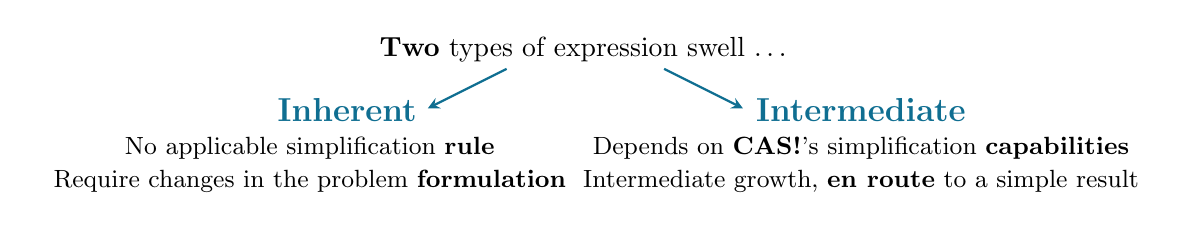
\begin{tikzpicture}[scale=0.5]
    \uncover<4->{\node at (0,0) {\textbf{Two} types of expression swell \dots};}
    \uncover<5->{\draw[fg_sl_color, thick, -stealth] (-2,-0.5) -- (-4.0,-1.5);
    \node at (-7,-2.5) {
      \begin{tabular}{c}
        \hi{\large ~~~~~~Inherent} \\
        \small{No applicable simplification \textbf{rule}} \\
        \small{Require changes in the problem \textbf{formulation}}
      \end{tabular}
    };}
    \uncover<6->{\draw[fg_sl_color, thick, -stealth] (+2,-0.5) -- (+4.0,-1.5);
    \node at (+7,-2.5) {
      \begin{tabular}{c}
        \hi{\large Intermediate} \\
        \small{Depends on \acs{CAS}'s simplification \textbf{capabilities}} \\
        \small{Intermediate growth, \textbf{en route} to a simple result}
      \end{tabular}
    };}
  \end{tikzpicture}}
\end{frame}

\subsection{\acl{LEM}}

\begin{frame}{\acl{LEM}}{Hierarchical Representation}
  We progressively \textbf{hide} complexity in veiling variables
  \begin{equation*}
    \begin{array}{c}
      \textcolor{mycolor1}{\underline{2xy(1+y)}} \cdot f(x,y) + \textcolor{mycolor2}{\underline{5z(3a+z)}} \cdot g(y) + \textcolor{mycolor3}{\underline{3c(xy+z)}} \cdot h(x,z) \\[0.1em]
      \textcolor{mycolor5}{\underline{v_1 \cdot f(x,y)}} + \textcolor{mycolor4}{\underline{v_2 \cdot g(y) + v_3 \cdot h(x,z)}} \\[0.1em]
      v_4 + v_5
    \end{array}
  \end{equation*}
  where the \textbf{veiling variables} are
  \begin{align*}
    \textcolor{mycolor1}{v_1} &= 2x(1+y) \\
    \textcolor{mycolor2}{v_2} &= 5z(3a+z) \\
    \textcolor{mycolor3}{v_3} &= 3c(xy+z) \\
    \textcolor{mycolor4}{v_4} &= \textcolor{mycolor1}{v_1} \cdot f(x,y) \\
    \textcolor{mycolor5}{v_5} &= \textcolor{mycolor2}{v_2} \cdot g(y) + \textcolor{mycolor3}{v_3} \cdot h(x,z)
  \end{align*}
\end{frame}

\begin{frame}{\acl{LEM}}{Hierarchical Representation}
  \uncover<1->{\textbf{Hierarchical representation} of expressions is performed through \textbf{veiling variables}
  \begin{equation*}
    \m{f}(\mx) \quad \autorightarrow{\text{veiling}}{\text{variables}} \quad \m{f}(\mx, \m{v})
    \qquad \text{where} \qquad
    \m{v}(\mx) = \msmall{\begin{bmatrix}
      v_{1}(\mx) \\
      v_{2}(v_{1}, \mx) \\
      \vdots \\
      v_{n}(v_{1}, \dots, v_{n-1}, \mx)
    \end{bmatrix}}
  \end{equation*}}
  \uncover<2->{The process is made of two actions \dots
  \begin{enumerate}
    \item a large expression can be \textbf{veiled} in a veiling variable
    \item veils can be \textbf{unveiled} to recover the original form
  \end{enumerate}}
  \vspace{0.5em}
  \uncover<3->{\hic{Complexity remains but the \acs{CAS} can not see it! \textcolor{fg_sl_color}{\large \faGlasses}}}
\end{frame}

\begin{frame}{\acl{LEM}}{Measuring Expression Complexity}
  \centering{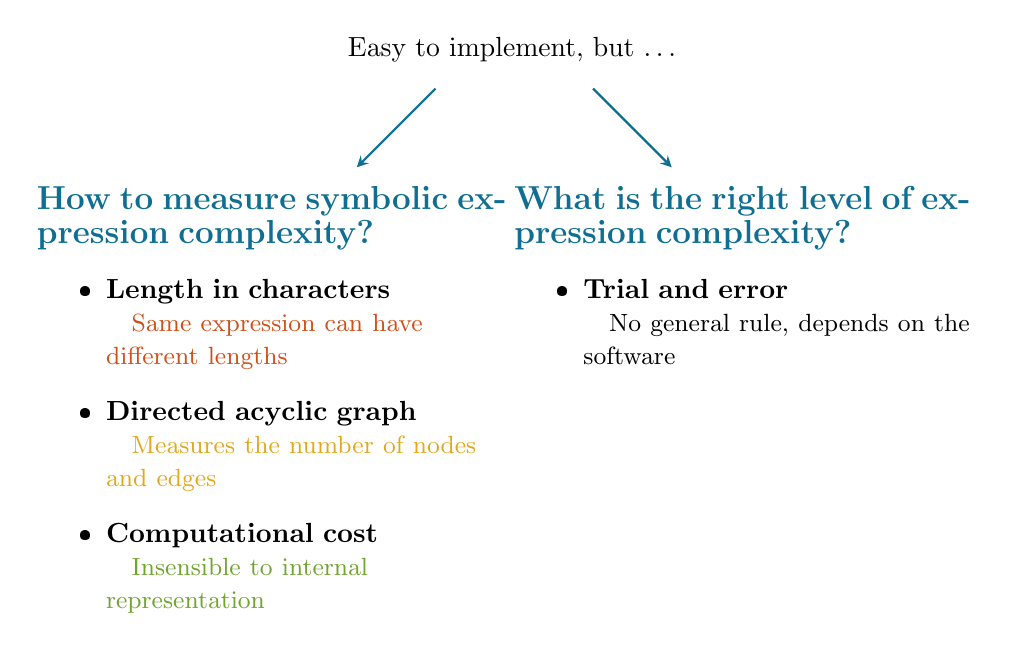
\begin{tikzpicture}[scale=0.5]
    \node at (0,0) {Easy to implement, but \dots};
    \uncover<1->{
      \draw[fg_sl_color, thick, -stealth] (-2,-1) -- (-4.0,-3);
      \draw (-0.5\textwidth,-3.25) node[below, text width=0.5\textwidth] {
      \hi{\large How to measure symbolic expression complexity?}
      \begin{itemize}
        \item \textbf{Length in characters} \\
        \begin{small}
          \quad \textcolor{mycolor2!95!black}{Same expression can have different lengths}
        \end{small}
        \item \textbf{Directed acyclic graph} \\
        \begin{small}
          \quad \textcolor{mycolor3!95!black}{Measures the number of nodes and edges}
        \end{small}
        \item \textbf{Computational cost} \\
        \begin{small}
          \quad \textcolor{mycolor5!95!black}{Insensible to internal representation}
        \end{small}
      \end{itemize}
    };}
    \uncover<2->{
      \draw[fg_sl_color, thick, -stealth] (+2,-1) -- (+4.0,-3);
      \draw (0.5\textwidth,-3.25) node[below, text width=0.5\textwidth] {
      \hi{\large What is the right level of expression complexity?}
      \begin{itemize}
        \item \textbf{Trial and error} \\
        \begin{small}
          \quad No general rule, depends on the software
        \end{small}
      \end{itemize}};
    }
  \end{tikzpicture}}
\end{frame}

\subsection{Symbolic Matrix Factorization}

\begin{frame}{Symbolic Matrix Factorization}{Considerations and Challenges}
  \hic{\faCanadianMapleLeaf~\Maple{} factorizations are sensitive to expression swell}
  \begin{itemize}
    \item<2-> \textbf{\acl{LU}~(\acs{LU})} and \textbf{\acl{FFLU}~(\acs{FFLU})} factorizations \dots \\
    \begin{small}
      \qquad preserve \textbf{sparsity} and \textbf{fill-in} \\
      \qquad perform \textbf{minimal algebraic manipulations} \\
      \qquad allow for custom \textbf{pivoting strategies}
    \end{small}
  \item<3->However\dots
    \begin{enumerate}
      \normalsize
      \item output's numerical stability is not guaranteed \\
      \begin{small}
        \qquad \textbf{How to ensure numerical stability?}
      \end{small}
      \item expressions grow unpredictably during manipulation \\
      \begin{small}
        \qquad \textbf{How to manage large symbolic expressions?}
      \end{small}
    \end{enumerate}
  \end{itemize}
\end{frame}

\begin{frame}{Symbolic Matrix Factorization}{Symbolic Pivoting Strategy}
  \vspace{-1.5em}
  \hic{How to ensure numerical stability?}
  \begin{columns}
    \begin{column}[c]{0.47\textwidth}
      A good symbolic \textbf{pivoting strategy} \dots
      \begin{enumerate}
        \item<1> selects the \textbf{minimum-degree} entry \\
        \begin{small}
          \qquad Limit fill-in
        \end{small}
        \item<2> if numeric, selects the \textbf{biggest} entry \\
        \begin{small}
          \qquad Improve numerical stability
        \end{small}
        \item<3> selects \textbf{least complicated} entry \\
        \begin{small}
          \qquad Limit expression swell
        \end{small}
        \item<4> looks for the \textbf{best choice} \\
        \begin{small}
          \qquad Full-pivoting strategy
        \end{small}
      \end{enumerate}
    \end{column}
    \begin{column}[c]{0.53\textwidth}
      \begin{algorithmic}\scriptsize
        \Procedure{SymbolicPivoting}{$\m{A}$, $k$}
        \State \only<1>{\hlc}{$\m{d}^r, \, \m{d}^c \gets \text{ComputeDegrees}(\m{A})$}
          \For{\only<4>{\hlc}{$i$ \textbf{from} $k$ \textbf{to} $m$}}
          \For{\only<4>{\hlc}{$j$ \textbf{from} $k$ \textbf{to} $n$}}
              \State $D_{ij} \gets \infty$
              \IfThen{$A_{ij} \neq 0$}
              {\only<1>{\hlc}{$D_{ij} \gets d^r_{i} \, \max(0, \, d^c_j-1) + d^c_j \, \max(0, \, d^r_i-1)$}}
            \EndFor
          \EndFor
          \State \only<1>{\hlc}{$\mathcal{P} \gets \text{Sort}(\m{D})$}
          \State $q, \, l \gets \, 0, \, 0$  and $p, \, p_c, \, p_n \gets \infty, \, \infty, \, \infty$
          \For{\textbf{all} $(i, j)$ \textbf{in} $\mathcal{P}$}
            \IfThen{$p_c \neq \infty$ \textbf{and} $D_{ij} > D_{ql}$}{\textbf{break}}
            \State $t \gets A_{ij}$
            \IfThen{$\text{Signature}(t) = 0$}{\textbf{continue}}
            \State $t \gets \text{Simplify}(t)$ and \only<3>{\hlc}{$t_c \gets \text{ExpressionComplexity}(t)$} and $t_n \gets \infty$
            \IfThen{$t$ is numeric}{\only<2>{\hlc}{$t_n \gets \max(1, \, \text{abs}(t))$}}
            \If{\only<3>{\hlc}{$t_c < p_c$} \textbf{or} (\only<2>{\hlc}{$t_c = p_c$} \textbf{and} \only<2>{\hlc}{$t_n > p_n$})}
              \State $q, \, l \gets i, \, j$ and $p, \, p_c, \, p_n \gets t, \, t_c, \, t_n$
            \EndIf
          \EndFor
          \State \textbf{return} $p, \, q, \, l$
        \EndProcedure
      \end{algorithmic}
    \end{column}
  \end{columns}
\end{frame}

\begin{frame}{Symbolic Matrix Factorization}{\acs{LEM} During Factorization}
  \vspace{-1.5em}
  \hic{How to manage large symbolic expressions?}
  \begin{columns}
    \begin{column}[c]{0.32\textwidth}
      Veils are introduced during \dots
      \begin{itemize}
        \item<1> \textbf{Factorization step} \\
        \begin{small}
          \qquad gaussian elimination \\
          \qquad Schur complement
        \end{small}
        \item<2> \textbf{Solution step} \\
        \begin{small}
          \qquad forward substitution \\
          \qquad backward substitution
        \end{small}
      \end{itemize}
    \end{column}
    \begin{column}[c]{0.36\textwidth}
      \uncover<1>{\begin{algorithmic}\scriptsize
        \Procedure{LU}{$\m{A}, \, k$}
          \State $\m{M} \gets \m{A}$
          \State $rnk \gets \min(m, \, n)$
          \For{$k$ \textbf{from} $1$ \textbf{to} $rnk$}
            \State $p, \, q, \, l \gets \text{SymbolicPivoting}(\m{M}, \, k)$
            \If{$p = 0$}
              \State $rnk \gets k-1$ and \textbf{break}
            \EndIf
            \State $\m{r}_k, \, \m{c}_k \gets \, q, \, l$
            \State $\m{M} \gets \text{SwapRowsCols}(\m{M}, \, k, \, q,  \, l)$
            \For{$i$ \textbf{from} $k+1$ \textbf{to} $m$}
              \State \only<1>{\hlc}{$M_{kk} \gets \text{Veil}(M_{kk})$}
              \State \only<1>{\hlc}{$M_{ik} \gets \text{Veil}(\text{Normalizer}(M_{ik}/M_{kk}))$}
              \For{$j$ \textbf{from} $k+1$ \textbf{to} $n$}
                \State \only<1>{\hlc}{$M_{ij} \gets \text{Veil}(\text{Normalizer}(M_{ij} - M_{ik}M_{kj}))$}
              \EndFor
            \EndFor
          \EndFor
          \State $\m{P}, \, \m{Q} \gets \text{PermutationMatrices}(\m{r}, \, \m{c})$
          \State $\m{L}, \, \m{U} \gets \text{LowerUpperMatrices}(\m{M})$
          \State \textbf{return} $\m{L}, \, \m{U}, \, \m{P}, \, \m{Q}, \, \m{r}, \, \m{c}, \, rnk$
        \EndProcedure
      \end{algorithmic}}
    \end{column}
    \begin{column}[c]{0.32\textwidth}
      \uncover<2>{\begin{algorithmic}\scriptsize
        \Procedure{SolveLU}{$\m{L}, \, \m{U}, \, \m{P}, \, \m{Q}, \, \m{b}$}
          \State $\m{y} \gets \m{P}\m{b}$
          \State $m, \, n \gets \text{Size}(\m{L})$
          \For{$i$ \textbf{from} $2$ \textbf{to} $m$}
            \State \only<2>{\hlc}{$y_i \gets \text{Veil}(y_i - \sum\nolimits_{j=1}^{i-1} L_{ij}y_j)$}
          \EndFor
          \State $x_n \gets \text{Veil}(y_n/U_{nn})$
          \For{$i$ \textbf{from} $n-1$ \textbf{to} $1$}
            \State \only<2>{\hlc}{$x_i \gets \text{Veil}(y_i - {\sum\nolimits_{j=i+1}^{n}} U_{ij}x_j)$}
            \State \only<2>{\hlc}{$x_i \gets \text{Veil}(x_i/U_{ii})$}
          \EndFor
          \State $\m{x} \gets \m{Q}^\top\m{x}$
        \EndProcedure
      \end{algorithmic}}
    \end{column}
  \end{columns}
\end{frame}

% That's all Folks!

%!TEX root = main.tex

\section{Index Reduction Algorithm}

\subsection{Separation of Differential and Algebraic Equations}

\begin{frame}{Index Reduction Algorithm}{Separation of Differential and Algebraic Equations}
  \vspace{-1.0em}
  \begin{columns}
    \begin{column}[c]{0.6\textwidth}
      \begin{enumerate}[<+->]
        \item Consider the \textbf{generic} \acsp{DAE} system
        \begin{equation*}
          \mF = \mA \mxp - \mb = \m{0}
        \end{equation*}
        \item \textbf{Separate} the equations with the cokernel $\mK$ and its orthogonal complement $\mN$ of $\mA$
        \begin{equation*}
          \begin{bmatrix} \mE \\ \m{0} \end{bmatrix} \mxp = \begin{bmatrix} \mg \\ \ma \end{bmatrix}
          ~~ \text{with} ~~
          \begin{array}{r@{~}c@{~}l}
            \mE &=& \mN \mA \\
            \mg &=& \mN \mb \\
            \ma &=& \mK \mb
          \end{array}
        \end{equation*}
      \end{enumerate}
      \vspace{-1.0em}
      \uncover<3->{\begin{bbox}[Cokernel Computation]
        The cokernel $\mK$ and its orthogonal complement $\mN$ of $\mA$ are calculated using matrix factorization
      \end{bbox}}
    \end{column}
    \begin{column}[c]{0.4\textwidth}
      \visible<3->{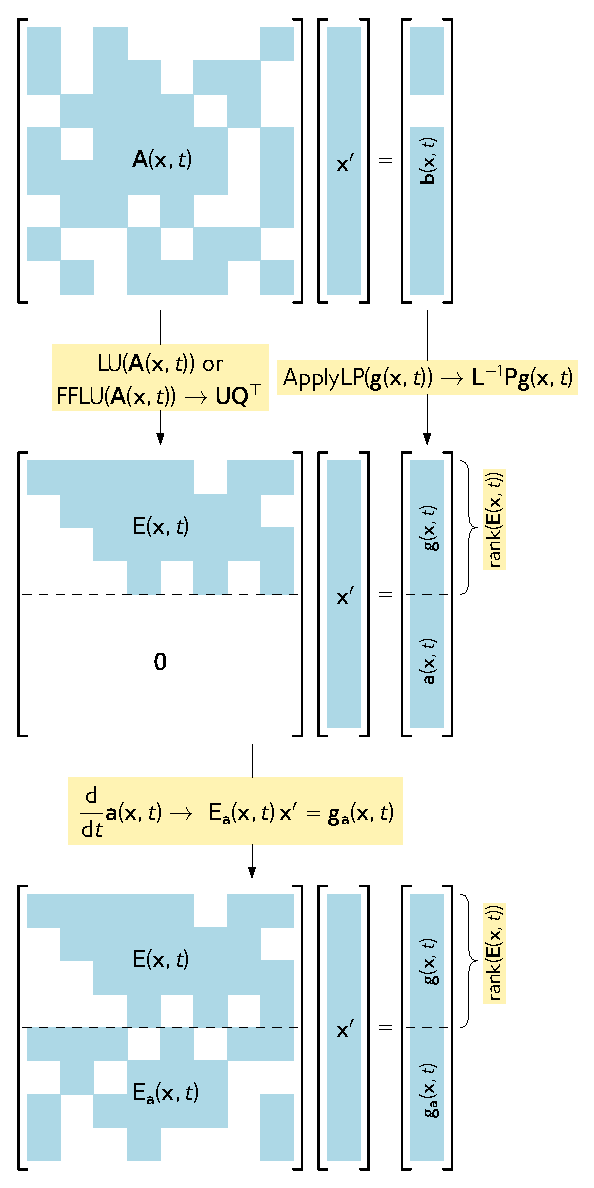
\includegraphics[width=1.0\textwidth, trim={0cm 7.35cm 0cm 0cm}, clip]{dae_visualization.eps}}
    \end{column}
  \end{columns}
\end{frame}

\subsection{Differentiation of Algebraic Equations}

\begin{frame}{Index Reduction Algorithm}{Differentiation of Algebraic Equations}
  \vspace{-1.5em}
  \begin{columns}
    \begin{column}[c]{0.6\textwidth}
      \begin{enumerate}[<+->]\setcounter{enumi}{2}
        \item Update the \textbf{invariants} as $\mh = \mh \cup \ma$
        \item \textbf{Differentiate} the algebraic equations $\ma$
        \begin{equation*}
          \dfrac{\text{d}}{\text{d}t} \ma = \mAd \mxp - \mgd
        \end{equation*}
        \item The \textbf{index reduced} system of \acsp{DAE} takes the form
        \begin{equation*}
          \begin{array}{c}
            \begin{bmatrix} \mE \\ \mAd \end{bmatrix}  \mxp =
            \begin{bmatrix} \mg \\ \mgd \end{bmatrix} \\[0.5em]
            \mF = \mA \mxp - \mb = \m{0}
            \end{array}
        \end{equation*}
      \end{enumerate}
      \uncover<3->{\begin{bbox}[A Sequential Algorithm]
        Apply \boxednumber{1}--\boxednumber{6} repeatedly until $\mA$ is non-singular
      \end{bbox}}
    \end{column}
    \begin{column}[c]{0.4\textwidth}
      \visible<2->{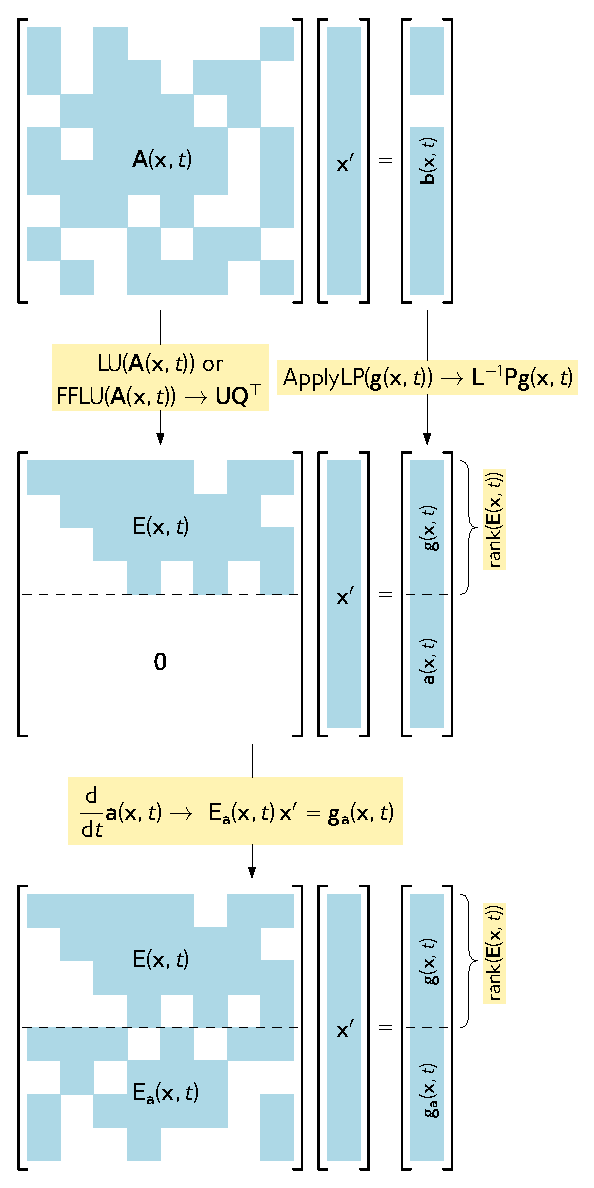
\includegraphics[width=1.0\textwidth, trim={0cm 0cm 0cm 7.35cm}, clip]{dae_visualization.eps}}
    \end{column}
  \end{columns}
\end{frame}

\begin{frame}{Index Reduction Algorithm}{Including Veiling Variables}
  \vspace{-1.0em}
  The algorithm can be extended to include \textbf{\acs{LEM}}
  \begin{itemize}
    \item veiling variables are stored in the list $\mv$
    \item equations are also function of $\mv$
    \item veiling variables add an evaluation layer to the algorithm
  \end{itemize}
  \vspace{-1.5em}\hspace{-0.025\textwidth}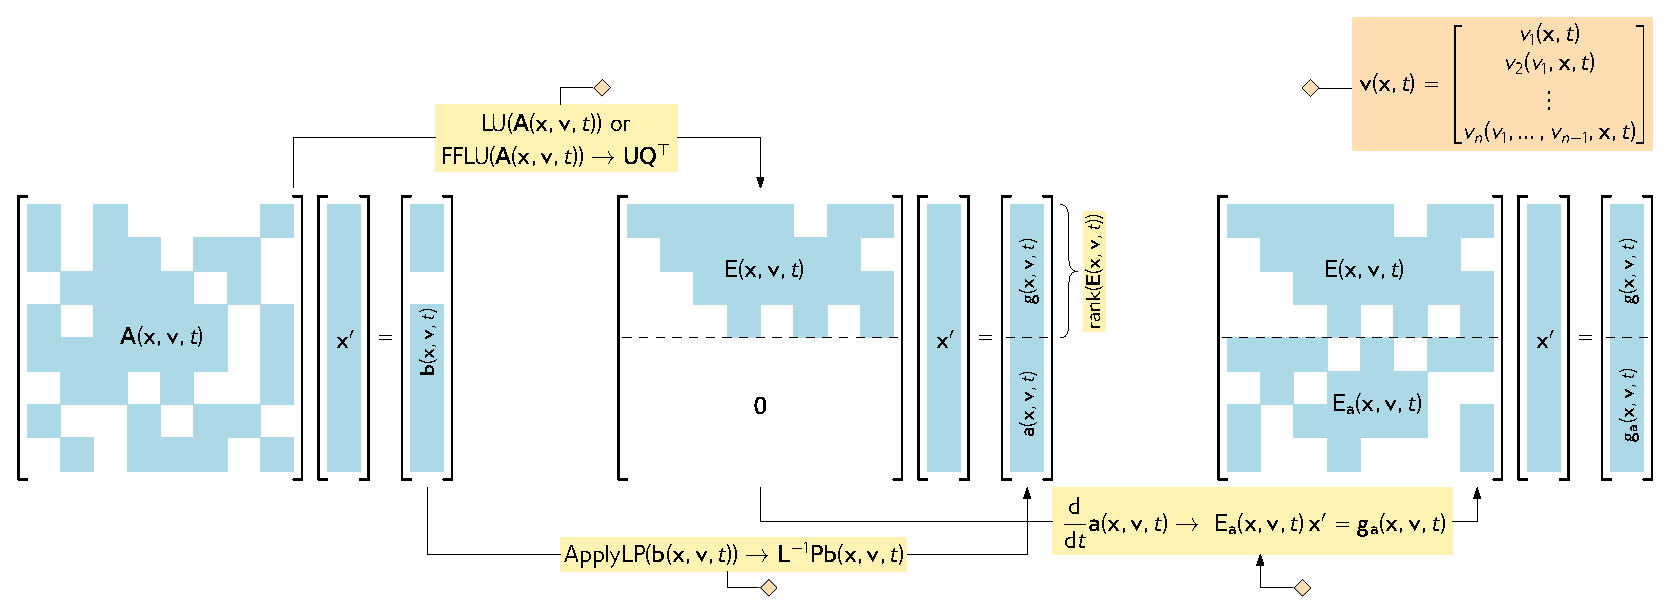
\includegraphics[width=1.05\textwidth]{dae_visualization_veil.eps}
\end{frame}

%\begin{frame}{Index Reduction Algorithm}{Algorithm Flowchart}
%  \centering
%  \begin{tikzpicture}[overlay]
%    \node at (0,0) {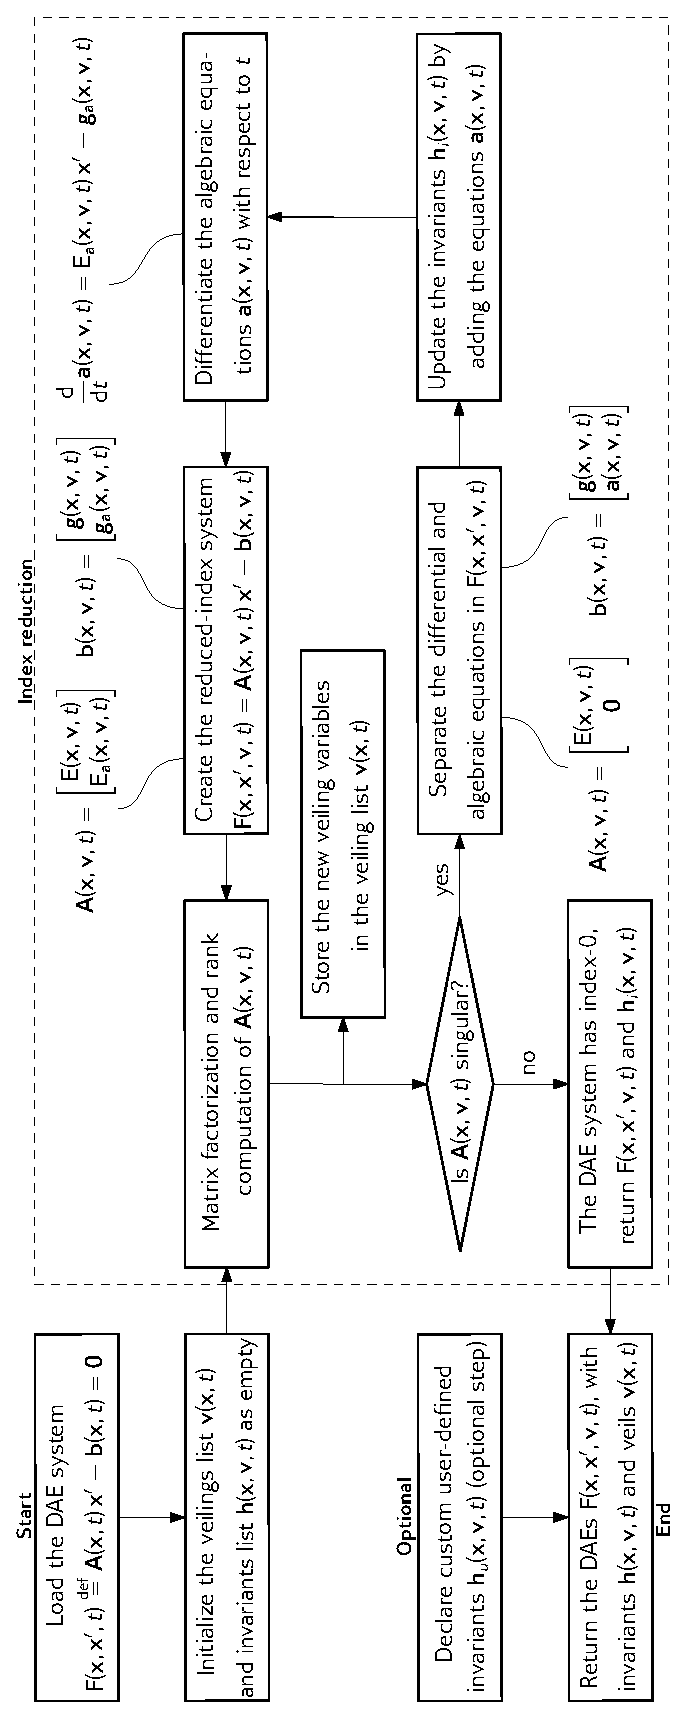
\includegraphics[angle=270, width=1.0\textwidth]{dae_flowchart_veil}};
%    \only<1>{\draw[fg_sl_color, line width=1.0pt] (-7.2,  2.9) rectangle (-3.7,  0.4);} % Initialization
%    \only<2>{\draw[fg_sl_color, line width=1.0pt] (-3.7,  2.9) rectangle ( 7.2, -2.9);} % Index Reduction
%    \only<3>{\draw[fg_sl_color, dashed, line width=1.0pt] (-7.2, -0.3) rectangle (-3.7, -1.6);} % Optional step
%    \only<4>{\draw[fg_sl_color, line width=1.0pt] (-7.2, -1.6) rectangle (-3.7, -2.9);} % Finalization
%  \end{tikzpicture}
%\end{frame}

\begin{frame}{Index Reduction Algorithm}{The Reduced \acs{DAE} System}
  \vspace{-1.0em}
  \hic{\faCanadianMapleLeaf~Now we can code-generate the reduced \acs{DAE} system!}
  \begin{itemize}[<+->]
    \item \textbf{Differential part}
    %
    \begin{equation*}
      \begin{array}{ccl}
          \m{F}(\mx, \mx^\prime, \m{v}, t) = \m{0} & \quad & \text{implicit  system class} \\
          \m{A}(\mx, \m{v}, t) \mx^\prime = \m{b}(\mx, \m{v}, t) & \quad & \text{semi-explicit system class} \\
          \mx^\prime = \m{f}(\mx, \m{v}, t) & \quad & \text{explicit system class}
      \end{array}
    \end{equation*}
    %
    \item \textbf{Invariants}
    %
    \begin{equation*}
      \m{h}(\mx, \m{v}, t) = \begin{bmatrix}
          \mhiv \\
          \mhuv
      \end{bmatrix} = \m{0} \quad \begin{array}{l}
        \text{hidden constraints} \\
        \text{\emph{optional} user-defined invariants}
        \end{array}
    \end{equation*}
    %
    \item \textbf{Veiling variables}
    %
    \begin{equation*}
        \m{v}(\mx, t) = \begin{bmatrix}
            v_{1}(\mx, t) \\
            v_{2}(v_{1}, \mx, t) \\
            \vdots \\
            v_{n}(v_{1}, \dots, v_{n-1}, \mx, t)
        \end{bmatrix}
    \end{equation*}
  \end{itemize}
\end{frame}

\subsection{Projection on Invariants}

\begin{frame}{Projection on Invariants}{Theoretical Background and Implementation}
  \vspace{-1.0em}
  \hic{\faAngleRight\hspace{-0.1em}\faAngleRight\hspace{-0.1em}\faAngleRight~Now we can integrate the system in \Matlab{}!}
  \begin{columns}
    \begin{column}[c]{0.6\textwidth}
      Projection is performed
      \begin{itemize}
        \item during the \textbf{numerical integration}
        \item to \textbf{enforce} the solution $\mx$ onto the $\mhv$ manifold
        \item by solving the \textbf{constrained minimization} problem
          \begin{align*}
            \underset{\mx}{\text{minimize}} \quad &\dfrac{1}{2}\left(\mx - \tilde{\mx}\right)^2 \\
            \text{subject to} \quad &\mhv = \m{0}
          \end{align*}
        \end{itemize}
      \end{column}
      \begin{column}[c]{0.4\textwidth}
        \hspace{-0.2\textwidth}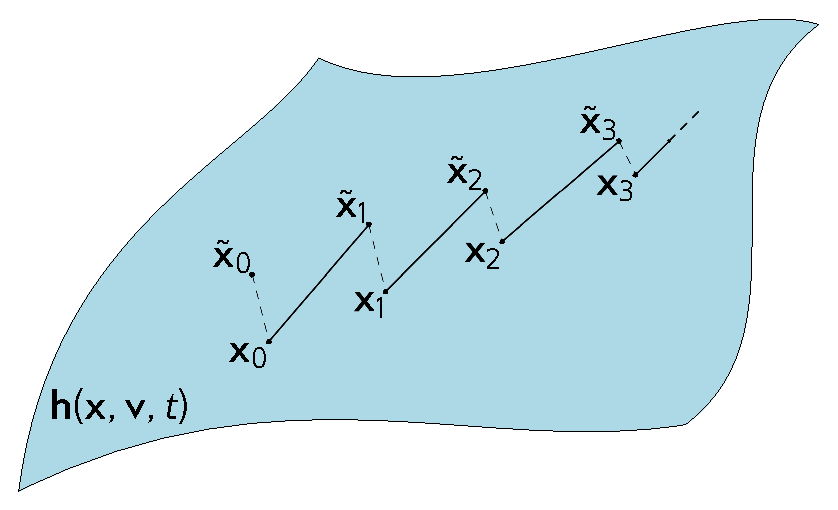
\includegraphics[width=1.2\textwidth]{projection.eps}
      \end{column}
    \end{columns}
    \vspace{1.0em}
    \hic{\large Find $\mx$ with minimal distance from $\tilde{\mx}$ that satisfies the invariants $\mhv$}
\end{frame}

%\begin{frame}{Projection on Invariants}{Theoretical Background and Implementation}
%  \begin{itemize}
%    \item The \textbf{Lagrangian} of the minimization problem is
%    \begin{equation*}
%      \mathcal{L}(\mx, \boldsymbol{\lambda}) = \frac{1}{2}\left(\mx - \tilde{\mx}\right)^2 + \boldsymbol{\lambda} \cdot \mhv
%      \quad \rightarrow \quad
%      \begin{cases}
%        \mx + \m{Jh}_\mx^\top \boldsymbol{\lambda} = \tilde{\mx} \\
%        \mhv = \m{0}
%      \end{cases}
%    \end{equation*}
%    \item The iterative method is \dots
%    \begin{equation*}
%      \begin{bmatrix}
%        \m{Jh}_{\mx} & \m{0} \\
%        \m{I}        & \m{Jh}_\mx^\top
%      \end{bmatrix}
%      \begin{bmatrix}
%        \delta\mx \\
%        \boldsymbol{\lambda}
%      \end{bmatrix} = \begin{bmatrix}
%        \tilde{\mx} - \mx \\
%        -\mhv
%      \end{bmatrix} \quad \text{where the step is} \quad \mx = \tilde{\mx} + \delta\mx
%    \end{equation*}
%    \item[] \dots derived from the \textbf{Taylor expansion}
%    \begin{equation*}
%      \begin{cases}
%        \mhv + \m{Jh}_{\mx}(\mx, \m{v}, t) \delta\mx + \textcolor{mycolor2}{\mathcal{O}\left(\| \delta\mx \|^2\right)} = \m{0} \\
%        \mx + \delta\mx + \m{Jh}_{\mx}^{\top}(\mx + \textcolor{mycolor2}{\delta \mx}, \m{v}, t) \boldsymbol{\lambda} = \tilde{\mx}
%      \end{cases}
%    \end{equation*}
%  \end{itemize}
%\end{frame}

\begin{frame}{Symbolic-Numerical Validation}{The Problem}
  \begin{columns}
    \begin{column}[c]{0.425\textwidth}
      A \textbf{particle} moving over a \textbf{torus} surface
      \begin{equation*}
        \begin{cases}
          x^{\prime}_{1} = u_{1} \\
          x^{\prime}_{2} = u_{2} \\
          x^{\prime}_{3} = u_{3} \\
          u^{\prime}_{1} = u_{3}\cos(t) - x_{3}\sin(t) - u_{2} + 2 c x_{1}\lambda \\
          u^{\prime}_{2} = u_{3}\sin(t) + x_{3}\cos(t) + u_{1} + 2 c x_{2}\lambda \\
          u^{\prime}_{3} = x_{3} + 2x_{3}\lambda \\
          \rho^2 = x_{1}^2 + x_{2}^2 + x_{3}^2 - 2r(x_{1}^2 + x_{2}^2)^{\frac{1}{2}} + r^2
        \end{cases}
      \end{equation*}
      with $c = 1 - r/(x_{1}^2 + x_{2}^2)^{\frac{1}{2}}$, $\rho = 5$, $r = 10$, and ICs $\mx_{0} = [15, 0, 0, 0, 15, -5, \lambda]^{\top}$
    \end{column}
    \begin{column}[c]{0.575\textwidth}
      \hic{\large Exact Solution}
      \begin{equation*}
        \mx_\text{exact} = \begin{bmatrix}
          x_{1} \\ x_{2} \\ x_{3}
        \end{bmatrix} = \begin{bmatrix}
          (\rho \cos(2\pi - t) + r) \cos(t) \\
          (\rho \cos(2\pi - t) + r) \sin(t) \\
          \rho \sin(2\pi - t)
        \end{bmatrix}
      \end{equation*} \\
      \centering{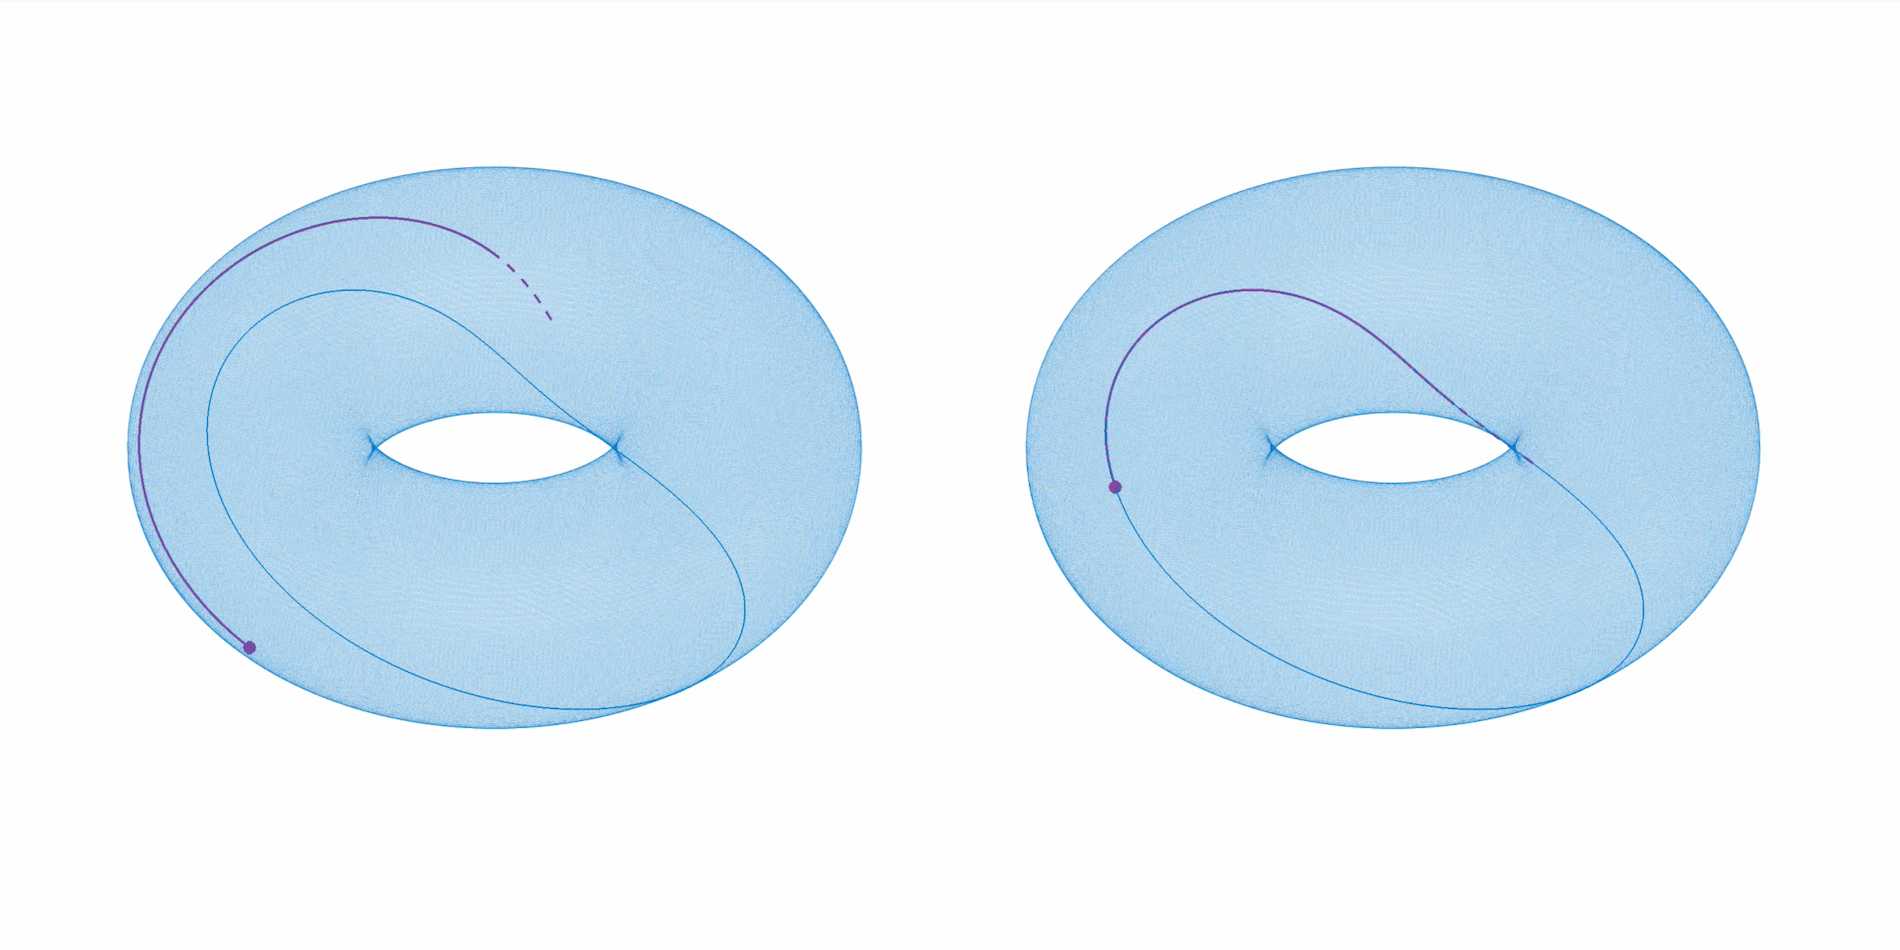
\includegraphics[width=0.6\textwidth, trim={17.0cm 3.5cm 2cm 2.5cm}, clip]{torus_3d_placeholder.png}}
    \end{column}
  \end{columns}
  \vspace{0.5em}
  \scriptsize{\fullcite{campbell1995constraint}}
\end{frame}

\begin{frame}{Symbolic-Numerical Validation}{Index Reduction}
  \vspace{-1.0em}
  \centering{\scriptsize\begin{tabular}{cccc}
    \multicolumn{4}{c}{\textbf{\acs{LU} Factorization}} \\
    \toprule
    \textbf{Original \acsp{DAE}} & \multicolumn{3}{c}{$\mF = 47\cf + 30\cm + 23\ca$ \quad $\mh = 0$} \\
    \midrule
    \textbf{Reduction step} & $\mE$ & $\mg$ & $\ma$ \\
    \midrule
    Index-3 \acsp{DAE} & $0$ & $39\cf + 36\cm + 13\ca$ & $7\cf + 10\cm + 6\ca$ \\
    Index-2 \acsp{DAE} & $0$ & $39\cf + 36\cm + 13\ca$ & $22\cf + 20\cm + 8\ca$ \\
    Index-1 \acsp{DAE} & $0$ & $39\cf + 36\cm + 13\ca$ & $68\cf + 72\cm + 33\ca$ \\
    Index-0 \acsp{DAE} & $388\cf + 424\cm + 180\ca$ & $79\cf + 77\cm + 26\ca$ & $0$ \\
    \midrule
    \rowcolor{mycolor5!25}
    \textbf{Reduced \acsp{DAE}} & \multicolumn{3}{c}{$\mF = 258\cf + 239\cm + 109\ca$ \quad $\mh = 97\cf + 102\cm + 47\ca$} \\
    \bottomrule \\[0.05em]
    %
    \multicolumn{4}{c}{\textbf{\acs{FFLU} Factorization}} \\
    \toprule
    \textbf{Original \acsp{DAE}} & \multicolumn{3}{c}{$\mF = 47\cf + 30\cm + 23\ca$ \quad $\mh = 0$} \\
    \midrule
    \textbf{Reduction step} & $\mE$ & $\mg$ & $\ma$ \\
    \midrule
    Index-3 \acsp{DAE} & $0$ & $39\cf + 36\cm + 13\ca$ & $7\cf + 10\cm + 6\ca$ \\
    Index-2 \acsp{DAE} & $0$ & $39\cf + 36\cm + 13\ca$ & $26\cf + 23\cm + 8\ca$ \\
    Index-1 \acsp{DAE} & $0$ & $39\cf + 36\cm + 13\ca$ & $68\cf + 72\cm + 33\ca$ \\
    Index-0 \acsp{DAE} & $388\cf + 424\cm + 180\ca$ & $79\cf + 77\cm + 26\ca$ & $0$ \\
    \midrule
    \rowcolor{mycolor2!25}
    \textbf{Reduced \acsp{DAE}} & \multicolumn{3}{c}{$\mF = 258\cf + 239\cm + 109\ca$ \quad $\mh = 101\cf + 105\cm + 47\ca$} \\
    \bottomrule \\[0.025em]
    \multicolumn{4}{c}{\small\emph{Legend}: $\cf$ = functions, $\ca$ = additions, $\cm$ = multiplications, and $\cd$ = divisions.}
    \end{tabular}}
\end{frame}

\begin{frame}{Symbolic-Numerical Validation}{Order and Error Analysis}
  \centering{\small{
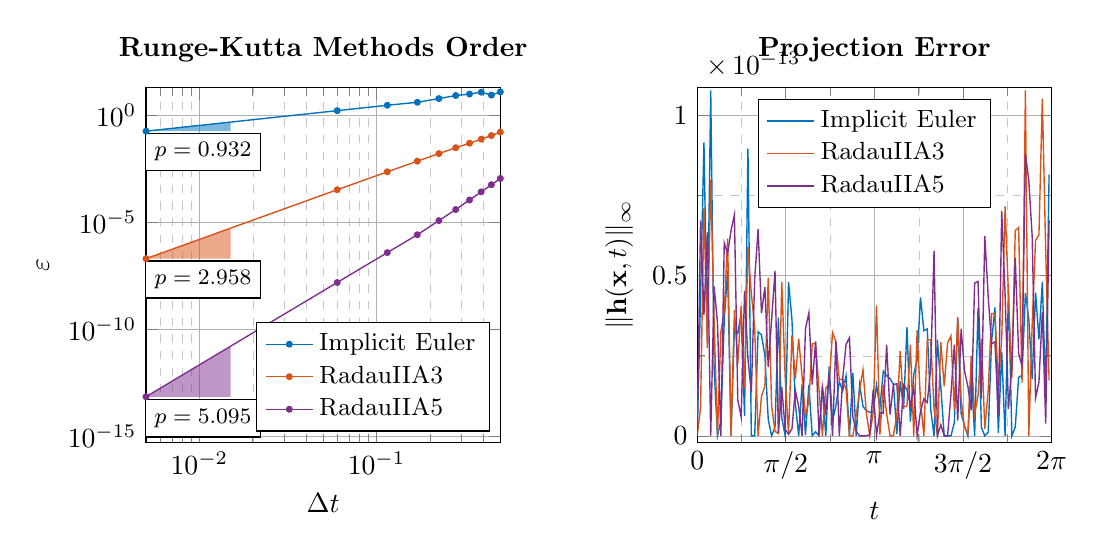
\begin{tikzpicture}

\begin{axis}[%
  title={Runge-Kutta Methods Order},
  title style={yshift=0.0mm, font=\bfseries},
  minor tick num=1,
  minor grid style={dashed, line width=0.1pt, draw=gray!45},
  major grid style={line width=0.2pt, draw=gray!60},
  width=4.5cm,
  height=4.5cm,
  at={(0.0in,0.0in)},
  scale only axis,
  xmode=log,
  xmin=0.005,
  xmax=0.5,
  xminorticks=true,
  xlabel style={font=\color{black}},
  xlabel={$\Delta t$},
  ymode=log,
  ymin=5.0e-16,
  ymax=20.0,
  yminorticks=true,
  ylabel style={font=\color{black}},
  ylabel={$\varepsilon$},
  axis background/.style={fill=none},
  xmajorgrids,
  xminorgrids,
  ymajorgrids,
  yminorgrids,
  legend style={font=\small, at={(0.97,0.03)}, anchor=south east, legend cell align=left, align=left, draw=black}
]

\addplot[color=mycolor1, line width=0.5pt, mark=*, mark options={fill, scale=0.5, mycolor1}]
  table[row sep=crcr]{%
  0.005 1.879399452620709e-01\\
  0.06 1.711573027753681e+00\\
  0.115 3.063916890081130e+00\\
  0.17 4.231237958056623e+00\\
  0.225 6.302317678343108e+00\\
  0.28 8.762767335676816e+00\\
  0.335 1.028329978855519e+01\\
  0.39 1.252649980402613e+01\\
  0.445 9.207336428245306e+00\\
  0.5 1.299428017259284e+01\\
};
\addlegendentry{Implicit Euler}

\addplot[color=mycolor2, line width=0.5pt, mark=*, mark options={fill, scale=0.5, mycolor2}]
  table[row sep=crcr]{%
  0.005 1.992528035899e-07\\
  0.06 0.000337631444430997\\
  0.115 0.00233186668661123\\
  0.17 0.00737183144006526\\
  0.225 0.0166514146938725\\
  0.28 0.0314018007261607\\
  0.335 0.0510617453643611\\
  0.39 0.0786646899717534\\
  0.445 0.11675270797915\\
  0.5 0.170354895882445\\
};
\addlegendentry{RadauIIA3}

\addplot[color=mycolor4, line width=0.5pt, mark=*, mark options={fill, scale=0.5, mycolor4}]
  table[row sep=crcr]{%
  0.005 6.75015598972095e-14\\
  0.06 1.52360311034272e-08\\
  0.115 3.82347098870639e-07\\
  0.17 2.62977937026676e-06\\
  0.225 1.20705485162631e-05\\
  0.28 3.98898559916816e-05\\
  0.335 0.000112061177007128\\
  0.39 0.000269397467860699\\
  0.445 0.000580087484554959\\
  0.5 0.00113800574884237\\
};
\addlegendentry{RadauIIA5}

\addplot[area legend, draw=none, fill=mycolor1, fill opacity=0.5, forget plot]
  table[row sep=crcr] {%
  x y\\
  0.005 0.187939945262071\\
  0.015 0.187939945262071\\
  0.015 0.494964142080998\\
}--cycle;

\addplot[area legend, draw=none, fill=mycolor2, fill opacity=0.5, forget plot]
  table[row sep=crcr] {%
  x y\\
  0.005 1.992528035899e-07\\
  0.015 1.992528035899e-07\\
  0.015 5.45505603722094e-06\\
}--cycle;

\addplot[area legend, draw=none, fill=mycolor4, fill opacity=0.5, forget plot]
  table[row sep=crcr] {%
  x y\\
  0.005 6.75015598972095e-14\\
  0.015 6.75015598972095e-14\\
  0.015 1.57024270189941e-11\\
}--cycle;

\node[draw, fill=white] at (1.05e-2, 2.00e-02) {\footnotesize{$p = 0.932$}};
\node[draw, fill=white] at (1.05e-2, 2.10e-08) {\footnotesize{$p = 2.958$}};
\node[draw, fill=white] at (1.05e-2, 0.65e-14) {\footnotesize{$p = 5.095$}};
\end{axis}

\begin{axis}[%
  title={Projection Error},
  title style={yshift=0.0mm, font=\bfseries},
  minor tick num=1,
  minor grid style={dashed, line width=0.1pt, draw=gray!45},
  major grid style={line width=0.2pt, draw=gray!60},
  width=4.5cm,
  height=4.5cm,
  at={(7.0cm,0.0in)},
  scale only axis,
  xmin=0,
  xmax=6.28318530717959,
  xlabel style={font=\color{black}},
  xlabel={$t$},
  xlabel shift={0.125em},
  xtick={0, 1.5707963267949, 3.14159265358979, 4.71238898038469, 6.28318530717959},
  xticklabels={$0$, $\pi/2$, $\pi$, $3\pi/2$, $2\pi$},
  %every y tick scale label/.style={
  %  at={(1.015, 0.945)}, anchor=south west, inner sep=0pt
  %},
  ytick scale label code/.code={$\times \, 10^{-13}$},
  ymin=-0.02e-13,
  ymax=1.085e-13,
  ylabel style={font=\color{black}},
  ylabel={$\| \mh \|_{\infty}$},
  %yticklabel pos=right,
  axis background/.style={fill=none},
  xmajorgrids,
  xminorgrids,
  ymajorgrids,
  yminorgrids,
  legend style={font=\small, at={(0.5,0.97)}, anchor=north, legend cell align=left, align=left, draw=black}
]

\addplot[color=mycolor1, line width=0.5pt]
  table[row sep=crcr]{%
  0.0	0\\
  0.06	4.34990500158268e-14\\
  0.12	9.14713630327889e-14\\
  0.18	2.98902106951307e-14\\
  0.24	1.07748232567088e-13\\
  0.3	2.10810383283768e-14\\
  0.36	0\\
  0.42	4.71502785877585e-15\\
  0.48	3.60007915114583e-14\\
  0.54	5.15958404494974e-14\\
  0.6	0\\
  0.66	3.37571546641056e-14\\
  0.72	3.20051218006002e-14\\
  0.78	3.81173776267159e-14\\
  0.84	6.1954391364817e-15\\
  0.9	8.95925122577517e-14\\
  0.96	0\\
  1.02	0\\
  1.08	3.24241260150387e-14\\
  1.14	3.14931663864555e-14\\
  1.2	2.50556225451883e-14\\
  1.26	5.09349295084449e-15\\
  1.32	0\\
  1.38	2.64245779923981e-15\\
  1.44	3.6842072004579e-14\\
  1.5	5.61897690710851e-15\\
  1.56	0\\
  1.62	4.8026106429562e-14\\
  1.68	3.63626524685878e-14\\
  1.74	1.01942880461704e-14\\
  1.8	0\\
  1.86	1.60069355130316e-14\\
  1.92	2.28518820214578e-16\\
  1.98	1.59079989935601e-14\\
  2.04	0\\
  2.1	1.27449819572632e-15\\
  2.16	0\\
  2.22	1.5182461883964e-14\\
  2.28	0\\
  2.34	2.15531930059804e-14\\
  2.4	4.76121391456162e-15\\
  2.46	9.36392103102618e-15\\
  2.52	1.68888906404432e-14\\
  2.58	1.40704033684351e-14\\
  2.64	1.86604175798768e-14\\
  2.7	0\\
  2.76	1.9584060661875e-14\\
  2.82	0\\
  2.88	1.59393949940154e-14\\
  2.94	9.17721100927432e-15\\
  3	7.80968852312227e-15\\
  3.06	7.388064091316e-15\\
  3.12	7.28584971153018e-15\\
  3.18	1.58906318290303e-14\\
  3.24	8.71670113035874e-15\\
  3.3	2.01335164715821e-14\\
  3.36	1.87429669449795e-14\\
  3.42	1.7813725413259e-14\\
  3.48	1.60851063568547e-14\\
  3.54	6.25687551665572e-16\\
  3.6	1.69547170411231e-14\\
  3.66	8.41775766141766e-15\\
  3.72	3.39216511899456e-14\\
  3.78	4.45866709099199e-15\\
  3.84	1.91680683420683e-14\\
  3.9	2.35877773802524e-14\\
  3.96	4.31470535972855e-14\\
  4.02	3.27790567623137e-14\\
  4.08	3.33643422441018e-14\\
  4.14	8.33060192023164e-15\\
  4.2	0\\
  4.26	2.99541085364436e-14\\
  4.32	1.53853495359176e-14\\
  4.38	0\\
  4.44	0\\
  4.5	0\\
  4.56	4.11555718048816e-15\\
  4.62	3.67780794600896e-14\\
  4.68	6.96692544670932e-15\\
  4.74	3.21649541394723e-15\\
  4.8	0\\
  4.86	1.98207634010965e-14\\
  4.92	0\\
  4.98	3.98983227546346e-14\\
  5.04	2.66738145006334e-15\\
  5.1	0\\
  5.16	1.14818597398386e-15\\
  5.22	2.94481485016782e-14\\
  5.28	4.00430584084634e-14\\
  5.34	8.39165155939648e-16\\
  5.4	2.62190029363372e-14\\
  5.46	0\\
  5.52	4.5388851313787e-14\\
  5.58	0\\
  5.64	2.69606312402563e-15\\
  5.7	1.82222934912061e-14\\
  5.76	1.89070359423442e-14\\
  5.82	4.45295027597655e-14\\
  5.88	3.65018441462149e-14\\
  5.94	1.76619003298675e-14\\
  6	4.4664737416553e-14\\
  6.06	3.00820691761593e-14\\
  6.12	4.79911837055461e-14\\
  6.18	1.29969770362389e-14\\
  6.24	8.14452283860879e-14\\
};\addlegendentry{Implicit Euler}

\addplot[color=mycolor2, line width=0.5pt]
  table[row sep=crcr]{%
  0	0\\
  0.06	8.84448873691838e-15\\
  0.12	7.10252993448526e-14\\
  0.18	2.73745627106684e-14\\
  0.24	7.98778880425246e-14\\
  0.3	3.6081075739454e-14\\
  0.36	0\\
  0.42	3.24265476848927e-14\\
  0.48	3.87046037491941e-14\\
  0.54	6.15239311809982e-14\\
  0.6	0\\
  0.66	3.91562582690368e-14\\
  0.72	2.25000036079271e-14\\
  0.78	4.04414271599053e-14\\
  0.84	1.49380061235967e-14\\
  0.9	5.89354034123046e-14\\
  0.96	4.43960827492856e-14\\
  1.02	3.38273659792399e-14\\
  1.08	0\\
  1.14	1.23582540282663e-14\\
  1.2	1.54714760360776e-14\\
  1.26	4.93042497956856e-14\\
  1.32	9.19872936629242e-15\\
  1.38	1.38615479184773e-15\\
  1.44	7.52495018973183e-16\\
  1.5	4.80001254407006e-14\\
  1.56	1.82980829289806e-14\\
  1.62	4.90034281627552e-16\\
  1.68	3.13259870821234e-14\\
  1.74	1.77625688404132e-14\\
  1.8	3.02811591570971e-14\\
  1.86	1.85416404827173e-14\\
  1.92	6.38757726249384e-15\\
  1.98	1.0616430615281e-14\\
  2.04	2.86913740347028e-14\\
  2.1	2.87532747854972e-14\\
  2.16	1.44908645537467e-14\\
  2.22	0\\
  2.28	1.48226453812946e-14\\
  2.34	1.6245848597906e-14\\
  2.4	3.22231789091681e-14\\
  2.46	2.92696331143997e-14\\
  2.52	1.74008700537511e-14\\
  2.58	1.77789685566004e-14\\
  2.64	1.44343986204923e-14\\
  2.7	0\\
  2.76	0\\
  2.82	6.40702877095534e-15\\
  2.88	1.42771571465927e-14\\
  2.94	2.0554256596902e-14\\
  3	7.06195117559697e-15\\
  3.06	0\\
  3.12	7.27089394097636e-15\\
  3.18	4.06350200553687e-14\\
  3.24	3.53559108943528e-16\\
  3.3	1.59074571212465e-14\\
  3.36	6.78088594942458e-15\\
  3.42	0\\
  3.48	0\\
  3.54	6.37313833585726e-15\\
  3.6	2.64233294813674e-14\\
  3.66	9.05705974224811e-15\\
  3.72	9.25806216032326e-15\\
  3.78	2.8421709430404e-14\\
  3.84	0\\
  3.9	3.29455139897558e-14\\
  3.96	1.07330281365035e-14\\
  4.02	0\\
  4.08	2.99993820655985e-14\\
  4.14	2.99302413301819e-14\\
  4.2	8.45649099423198e-15\\
  4.26	0\\
  4.32	2.92414129726747e-14\\
  4.38	1.55071468737394e-14\\
  4.44	2.89702385935865e-14\\
  4.5	3.11590712535806e-14\\
  4.56	8.06643782767062e-15\\
  4.62	3.71860560727394e-14\\
  4.68	1.15774417663157e-14\\
  4.74	2.40000466840985e-15\\
  4.8	7.99747337593166e-16\\
  4.86	2.49901770525562e-14\\
  4.92	6.77554661163664e-15\\
  4.98	1.2538207925704e-14\\
  5.04	3.03245905494408e-14\\
  5.1	2.16408472173715e-15\\
  5.16	1.40062502346563e-14\\
  5.22	3.81524411539504e-14\\
  5.28	3.8071688841407e-14\\
  5.34	1.57202927985259e-14\\
  5.4	3.0377210200149e-14\\
  5.46	7.15590051863223e-14\\
  5.52	4.38239782516872e-14\\
  5.58	1.79951982640777e-14\\
  5.64	6.39867062902223e-14\\
  5.7	6.49615736545083e-14\\
  5.76	1.66177595708798e-14\\
  5.82	1.07695444051526e-13\\
  5.88	0\\
  5.94	3.46718274762021e-14\\
  6	6.08947400862772e-14\\
  6.06	6.27262279676494e-14\\
  6.12	1.05156307287711e-13\\
  6.18	5.75007020364114e-14\\
  6.24	1.72627172653053e-14\\
};
\addlegendentry{RadauIIA3}

\addplot[color=mycolor4, line width=0.5pt]
  table[row sep=crcr]{%
  0	0\\
  0.06	6.71403541230021e-14\\
  0.12	3.77283965133535e-14\\
  0.18	6.34330992622269e-14\\
  0.24	0\\
  0.3	4.65706896752599e-14\\
  0.36	3.53024518099557e-14\\
  0.42	0\\
  0.48	6.01556977798936e-14\\
  0.54	5.6843418860808e-14\\
  0.6	6.3998447010507e-14\\
  0.66	6.89462466735111e-14\\
  0.72	1.11734380999568e-14\\
  0.78	5.84336673739155e-15\\
  0.84	4.51547342643318e-14\\
  0.9	2.40345531292498e-14\\
  0.96	1.35285891842221e-14\\
  1.02	4.89969933702126e-14\\
  1.08	6.44519721994705e-14\\
  1.14	3.82027084757365e-14\\
  1.2	4.63610229041449e-14\\
  1.26	2.14012786085607e-14\\
  1.32	3.62129381964501e-14\\
  1.38	5.14278476238434e-14\\
  1.44	7.52475217963951e-16\\
  1.5	1.51595717211594e-14\\
  1.56	2.01357850117944e-15\\
  1.62	4.90016969470829e-16\\
  1.68	2.15197114109576e-15\\
  1.74	1.42094637215295e-14\\
  1.8	9.14135367252492e-15\\
  1.86	0\\
  1.92	3.33136607299302e-14\\
  1.98	3.83629683826335e-14\\
  2.04	1.59967695360947e-14\\
  2.1	2.94212446823591e-14\\
  2.16	0\\
  2.22	1.51864101443109e-14\\
  2.28	7.27563915445106e-15\\
  2.34	1.93360441784085e-14\\
  2.4	0\\
  2.46	2.9511735315762e-14\\
  2.52	0\\
  2.58	1.77786569080783e-14\\
  2.64	2.85341341331248e-14\\
  2.7	3.06062249475849e-14\\
  2.76	6.05430255954215e-15\\
  2.82	1.35178386471263e-15\\
  2.88	0\\
  2.94	0\\
  3	0\\
  3.06	3.54093358009643e-16\\
  3.12	1.42133513334771e-14\\
  3.18	1.77504779217282e-16\\
  3.24	7.24938179967691e-15\\
  3.3	7.00937076054701e-15\\
  3.36	2.84301825312368e-14\\
  3.42	6.63882013161966e-15\\
  3.48	1.6007712487894e-14\\
  3.54	1.62299374575982e-14\\
  3.6	0\\
  3.66	1.58874434059998e-14\\
  3.72	1.44195741501297e-14\\
  3.78	9.49801118770299e-15\\
  3.84	1.49386437805692e-14\\
  3.9	0\\
  3.96	7.70015247254448e-15\\
  4.02	1.15286998476027e-14\\
  4.08	1.04060301103914e-14\\
  4.14	2.10957320580662e-14\\
  4.2	5.76430753406985e-14\\
  4.26	0\\
  4.32	3.43798720861495e-15\\
  4.38	0\\
  4.44	0\\
  4.5	1.29595646328969e-14\\
  4.56	2.84138752512645e-14\\
  4.62	4.71567077252452e-15\\
  4.68	3.33738140247112e-14\\
  4.74	2.02937095842527e-14\\
  4.8	1.53930076582013e-14\\
  4.86	7.91332496467288e-15\\
  4.92	4.76635995797504e-14\\
  4.98	4.81895564192324e-14\\
  5.04	1.16266826302188e-14\\
  5.1	6.2319428928642e-14\\
  5.16	4.3455302159109e-14\\
  5.22	2.86730496772646e-14\\
  5.28	2.9300964947864e-14\\
  5.34	6.72223560445336e-15\\
  5.4	7.0170982385832e-14\\
  5.46	4.40352521641556e-14\\
  5.52	8.35122710587472e-15\\
  5.58	2.20814842274086e-14\\
  5.64	5.55417576536816e-14\\
  5.7	2.55536510002858e-14\\
  5.76	2.1865754534927e-14\\
  5.82	8.783763173108e-14\\
  5.88	7.96680804218409e-14\\
  5.94	6.22830583836424e-14\\
  6	1.18139987543405e-14\\
  6.06	1.67364446109691e-14\\
  6.12	3.86667246627752e-14\\
  6.18	3.79629193314912e-15\\
  6.24	6.70788729037476e-14\\
};
\addlegendentry{RadauIIA5}

\end{axis}

\end{tikzpicture}%}}
\end{frame}

\begin{frame}{Symbolic-Numerical Validation}{Solution Visualization}
  \vspace{-1.0em}
  \hic{RadauIIA5 \quad $\Delta t = 0.05$\,s \quad $t \in [0, 200\pi]$\,s}
  \vspace{1.0em}
  \centering\small
  \textbf{No projection}%
  \hspace{10.0em}%
  \textbf{With projection}
  \movie[label=show1, width=0.8\textwidth, autostart, poster, showcontrols, loop]{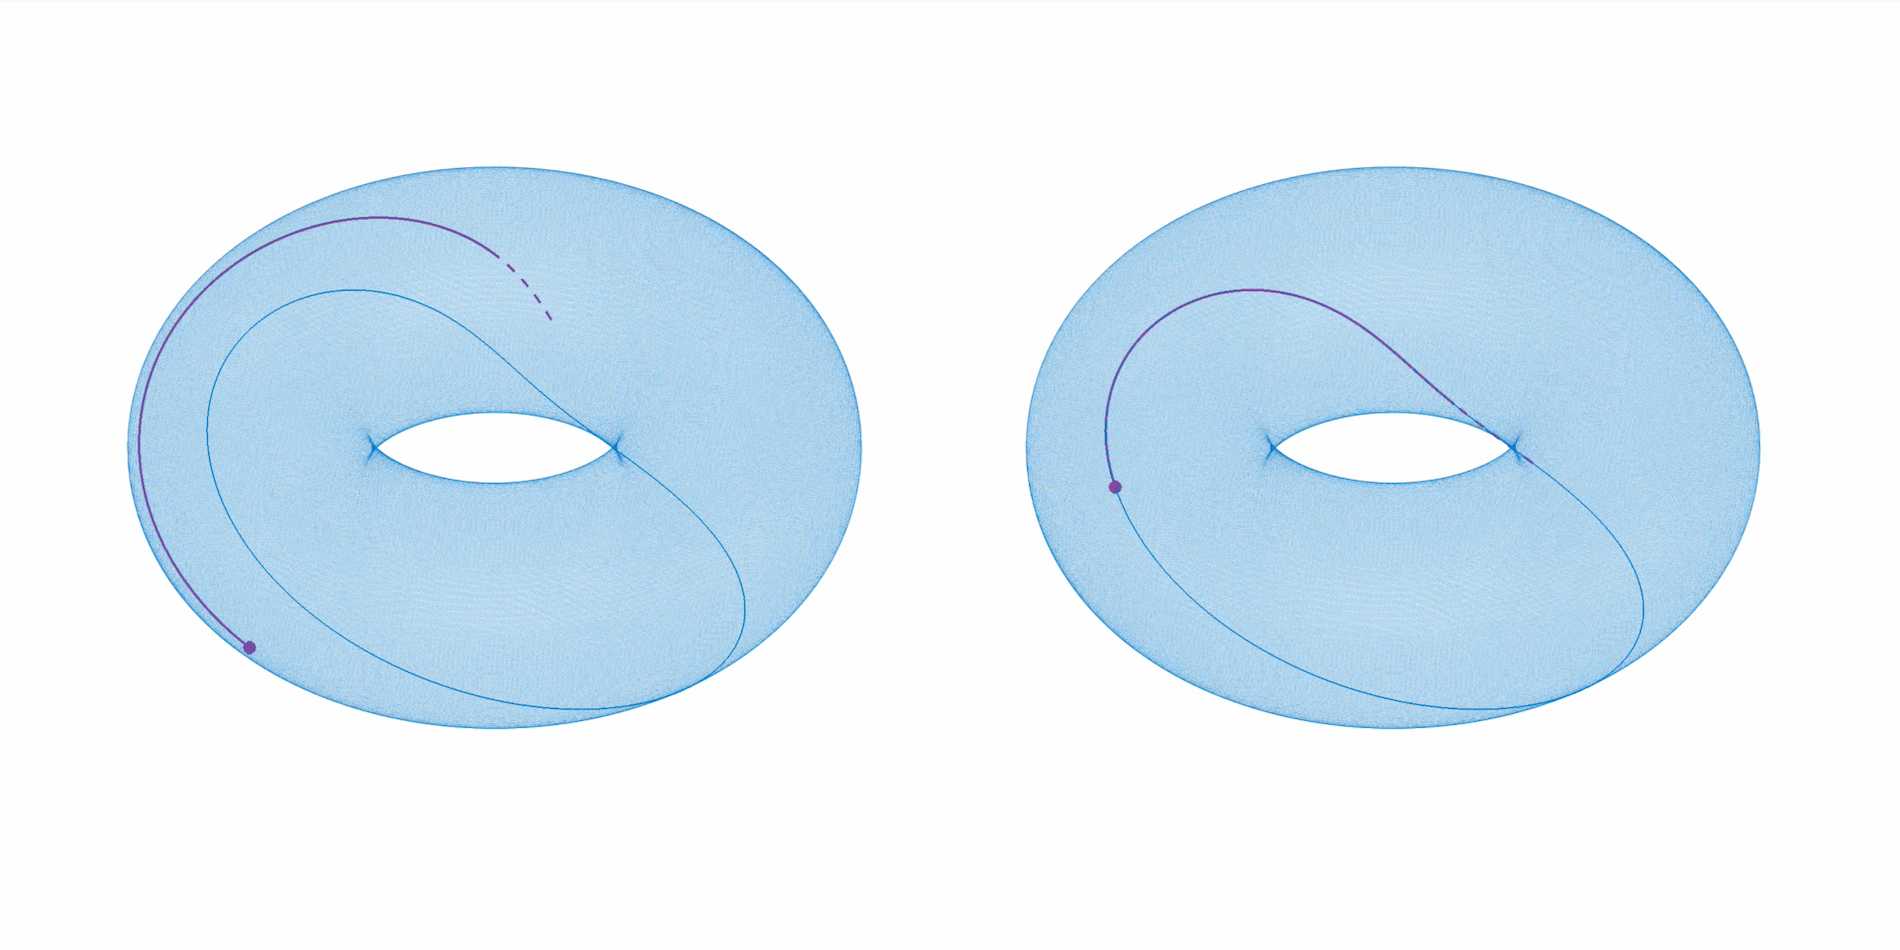
\includegraphics[width=0.8\textwidth]{torus_3d_placeholder.png}}{movie/torus_3d.mov}
\end{frame}

% That's all Folks!
%!TEX root = main.tex

\section{Application Fields and Examples}

\begin{frame}{Application Fields and Examples}{Bechmarking the Index Reduction Algorithm}
  \begin{columns}
    \begin{column}[c]{0.4\textwidth}
      The \textbf{benchmarks} \dots
      \begin{itemize}
        \item Multi-body dynamics:
        \begin{enumerate}\scriptsize
          \item Car-axis;
          \item Flexible slider-crank;
          \item Double-wishbone suspension.
        \end{enumerate}
        \item Trajectory prescribed path control problems:
        \begin{enumerate}\setcounter{enumi}{3}\scriptsize
          \item Space shuttle reentry (initial stage);
          \item Space shuttle reentry (final stage);
          \item Robotic arm control.
        \end{enumerate}
        \item Electric Circuits:
        \begin{enumerate}\setcounter{enumi}{6}\scriptsize
          \item Eight-nodes transistor-amplifier;
          \item Electric ring modulator;
          \item Cascaded differential amplifiers.
        \end{enumerate}
        \item Generic \ac{DAE} systems:
        \begin{enumerate}\setcounter{enumi}{9}\scriptsize
          \item Particle motion;
          \item $N$-pendula ($N = 2, 3, 4, 5$).
        \end{enumerate}
      \end{itemize}
    \end{column}
    \begin{column}[c]{0.6\textwidth}
      The \textbf{competitors} \dots
      \begin{itemize}
        \item \Maple{}'s \texttt{dsolve} (undisclosed);
        \item \Matlab{}'s \texttt{reduceDAEIndex} (Pantelides)
        \item \Matlab{}'s \texttt{reduceDAEToODE} (Gaussian elimination)
        \item \Mathematica{}'s \texttt{NDSolve} (Pantelides)
      \end{itemize}
      \vspace{1.0em}
      The \textbf{rules} \dots
      \begin{itemize}
        \item \SI{100}{\second} time limit for symbolic simplification;
        \item Unlimited time for numerical integration;
        \item If you can integrate the problem, you lose.
      \end{itemize}
    \end{column}
  \end{columns}
\end{frame}

\begin{frame}{Application Fields and Examples}{Factorizations Performance}
  \vspace{-1.5em}
  \hic{\ac{LU} performed slightly better than \ac{FFLU}.}
  \centering{\scriptsize\begin{tabular}{cccc}
    \multicolumn{4}{c}{\textbf{Car-Axis (Index-3) -- \ac{LU} Factorization}} \\
    \toprule
    \textbf{Original \acp{DAE}} & \multicolumn{3}{c}{$\mF = 108\cf + 131\cm + 56\ca$ \quad $\mh = 0$} \\
    \midrule
    \textbf{Reduction step} & $\mE$ & $\mg$ & $\ma$ \\
    \midrule
    Index-3 \acp{DAE} & $12\cm$ & $94\cf + 145\cm + 54\ca$ & $14\cf + 16\cm + 10\ca$ \\
    Index-2 \acp{DAE} & $12\cm$ & $94\cf + 145\cm + 54\ca$ & $26\cf + 45\cm + 15\ca$ \\
    Index-1 \acp{DAE} & $12\cm$ & $94\cf + 145\cm + 54\ca$ & $136\cf + 4\cd + 261\cm + 95\ca$ \\
    Index-0 \acp{DAE} & $1060\cf + 38\cd + 1901\cm + 717\ca$ & $431\cf + 8\cd + 842\cm + 268\ca$ & $0$ \\
    \midrule
    \textbf{Reduced \acp{DAE}} & \multicolumn{3}{c}{$\mF = 896\cf + 4\cd + 1202\cm + 546\ca$ \quad $\mh = 176\cf + 4\cd + 322\cm + 120\ca$} \\
    \bottomrule \\[0.05em]
    %
    \multicolumn{4}{c}{\textbf{Car-Axis (Index-3) -- \ac{FFLU} Factorization}} \\
    \toprule
    \textbf{Original \acp{DAE}} & \multicolumn{3}{c}{$\mF = 108\cf + 131\cm + 56\ca$ \quad $\mh = 0$} \\
    \midrule
    \textbf{Reduction step} & $\mE$ & $\mg$ & $\ma$ \\
    \midrule
    Index-3 \acp{DAE} & $0$ & $94\cf + 8\cd + 150\cm + 54\ca$ & $14\cf + 21\cm + 10\ca$ \\
    Index-2 \acp{DAE} & $0$ & $94\cf + 8\cd + 154\cm + 54\ca$ & $26\cf + 1\cd + 44\cm + 15\ca$ \\
    Index-1 \acp{DAE} & $0$ & $94\cf + 8\cd + 155\cm + 54\ca$ & $136\cf + 6\cd + 4\cd + 261\cm + 95\ca$ \\
    Index-0 \acp{DAE} & $1066\cf + 55\cd + 1888\cm + 717\ca$ & $431\cf + 18\cd + 851\cm + 268\ca$ & $0$ \\
    \midrule
    \textbf{Reduced \acp{DAE}} & \multicolumn{3}{c}{$\mF = 1549\cf + 73\cd + 2765\cm + 1011\ca$ \quad $\mh = 176\cf + 7\cd + 326\cm + 120\ca$} \\
    \bottomrule
  \end{tabular}}
\end{frame}

\begin{frame}{Application Fields and Examples}{Expression Swell}
  \hic{Strong expression swell may still arise \dots}
  \hspace{-2.0em}
  \centering{\scriptsize\begin{tabular}{cccc}
    \multicolumn{4}{c}{\textbf{Robotic Arm (Index-5)}} \\
    \toprule
    \textbf{Original \acp{DAE}} & \multicolumn{3}{c}{$\mF = 125\cf + 19\cd + 56\cm + 64\ca$ \quad $\mh = 0$} \\
    \midrule
    \textbf{Reduction step} & $\mE$ & $\mg$ & $\ma$ \\
    \midrule
    Index-5 \acp{DAE} & $0$ & $66\cf + 3\cd + 50\cm + 35\ca$ & $16\cf + 12\ca$ \\
    Index-4 \acp{DAE} & $0$ & $66\cf + 3\cd + 50\cm + 35\ca$ & $24\cf + 6\cm + 14\ca$ \\
    Index-3 \acp{DAE} & $0$ & $66\cf + 3\cd + 50\cm + 35\ca$ & $162\cf + 2\cd + 138\cm + 114\ca$ \\
    Index-2 \acp{DAE} & $14\cf + 2\cd + 6\cm + 6\ca$ & $372\cf + 4\cd + 375\cm + 253\ca$ & $972\cf + 1\cd + 1062\cm + 770\ca$ \\
    \rowcolor{mycolor2!25}
    Index-1 \acp{DAE} & $14\cf + 2\cd + 6\cm + 6\ca$ & $372\cf + 4\cd + 375\cm + 253\ca$ & $\star (6.5\cf + 5.6\cm + 1.8\ca)\!\cdot\!10^{6} + 4\cd$ \\
    \rowcolor{mycolor2!25}
    Index-0 \acp{DAE} & $\star (8.3\cf + 7.1\cm + 2.3\ca)\!\cdot\!10^{7} + 58\cd$ & $(2.4\cf + 2.0\cm + 0.9\ca)\!\cdot\!10^{6} + 8\cd$ & $0$ \\
    \midrule
    \rowcolor{mycolor2!25}
    \textbf{Reduced \acp{DAE}} & \multicolumn{3}{c}{$\star \mF = (8.6\cf + 7.3\cm + 2.4\ca)\!\cdot\!10^{7} + 66\cd$ \quad $\star \mh = (6.5\cf + 5.6\cm + 1.8\ca)\!\cdot\!10^{6} + 7\cd$} \\
    \bottomrule
    \end{tabular}}
\end{frame}

\begin{frame}{Application Fields and Examples}{Expression Swell}
  \vspace{-2.0em}
  \hic{\dots Even using hierarchical representation.}
  \vspace{-0.5em}
  \centering{\scriptsize\begin{tabular}{cccc}
    \multicolumn{4}{c}{\textbf{Robotic Arm (Index-5)}} \\
    \toprule
    \textbf{Original \acp{DAE}} & \multicolumn{3}{c}{$\mFv = 125\cf + 19\cd + 56\cm + 64\ca$ \quad $\mhv = 0$ \quad $\mv = 0$} \\
    \midrule
    \textbf{Reduction step} & $\mEv$ & $\mgv$ & $\mav$ \\
    \midrule
    Index-5 \acp{DAE} & $0$ & $66\cf + 3\cd + 50\cm + 35\ca$ & $16\cf + 12\ca$ \\
    Index-4 \acp{DAE} & $0$ & $66\cf + 3\cd + 50\cm + 35\ca$ & $24\cf + 6\cm + 14\ca$ \\
    Index-3 \acp{DAE} & $0$ & $66\cf + 3\cd + 50\cm + 35\ca$ & $162\cf + 2\cd + 138\cm + 114\ca$ \\
    Index-2 \acp{DAE} & $14\cf + 2\cd + 6\cm + 6\ca$ & $66\cf + 1\cv + 3\cd + 51\cm + 35\ca$ & $1\cm + 1\cv$ \\
    \rowcolor{mycolor5!25}
    Index-1 \acp{DAE} & $2\cv + 1\ca$ & $66\cf + 1\cv + 3\cd + 51\cm + 35\ca$ & \cellcolor{mycolor5!25}$9\cf + 4\cv + 2\cd + 8\cm + 5\ca$ \\
    \rowcolor{mycolor5!25}
    Index-0 \acp{DAE} & $7\cv + 1\cd + 2\cm + 2\ca$ & \cellcolor{mycolor5!25}$66\cf + 2\cv + 3\cd + 52\cm + 35\ca$ & $0$ \\
    \midrule
    \rowcolor{mycolor5!25}
    \textbf{Reduced \acp{DAE}} & \multicolumn{3}{c}{$\mFv = 90\cf + 9\cv + 4\cd + 63\cm + 48\ca$ \quad $\mhv = 202\cf + 5\cv + 4\cd + 141\cm + 130\ca$} \\
    \bottomrule \\[-0.65em]
  \end{tabular}}
  \centering{\scriptsize\begin{tabular}{cc}
    \multicolumn{2}{c}{Hierarchical representation details (29 veils)} \\
    \toprule
    \textbf{Reduction step} & $\mv$ \\
    \midrule
    Index-5 \acp{DAE} & $0$ \\
    Index-4 \acp{DAE} & $0$ \\
    Index-3 \acp{DAE} & $0$ \\
    Index-2 \acp{DAE} & $1278\cf + 3\cv + 6\cd + 1319\cm + 918\ca$ \\
    \rowcolor{mycolor3!25}
    Index-1 \acp{DAE} & $8401\cf + 20\cv + 24\cd + 9451\cm + 6095\ca$ \\
    \rowcolor{mycolor3!25}
    Index-0 \acp{DAE} & $37010\cf + 558\cv + 56\cd + 45087\cm + 28665\ca$ \\
    \midrule
    \rowcolor{mycolor3!25}
    \textbf{Reduced \acp{DAE}} & $\mv = 37010\cf + 558\cv + 56\cd + 45087\cm + 28665\ca$ \\
    \bottomrule
  \end{tabular}}
\end{frame}

\begin{frame}{Application Fields and Examples}{Numerical Stability}

\end{frame}

\begin{frame}{Application Fields and Examples}{Expression Swell}
\end{frame}

% That's all Folks!
%!TEX root = main.tex

\section{Conclusions}

\begin{frame}{Possible Improvements}
    \uncover<1-3>{\hi{Index Reduction}}
    \begin{enumerate}
      \item<1> Detection of \textbf{linear index-1 variables}, similar to the \acs{MBD} case
      \begin{equation*}
        \begin{cases}
          \m{q}^{\prime} = \m{p} \\
          \m{p}^{\prime} = \dot{\m{p}}
        \end{cases}
        \text{where} \quad
        \begin{bmatrix}
          \m{M}(\m{q}, \m{p}, t)      & -\boldsymbol{\Phi}_{\m{q}}(\m{q}, t)^{\top} \\
          -\boldsymbol{\Phi}_{\m{q}}(\m{q}, t) & \m{0}
        \end{bmatrix}
        \begin{bmatrix}
          \dot{\m{p}} \\ \boldsymbol{\lambda}
        \end{bmatrix} = \begin{bmatrix}
          \m{f}(\m{q}, \m{p}, t) \\
          \dot{\boldsymbol{\Phi}}_{\m{q}}(\m{q}, t)\m{p} + \boldsymbol{\Phi}_{tt}(\m{q}, t)
        \end{bmatrix}
      \end{equation*}
      \item<2> \textbf{System augmentation} with ``veil'' equations \\
      \begin{small}
        \qquad complicated pivots become ``veil'' equations \\
        \qquad 1s in the diagonal, complicated terms on the RHS
      \end{small}
      \item<3> \textbf{Open-source} \acs{CAS} \\
      \begin{small}
        \qquad what is happening inside? \\
        \qquad why is it not working on this example?
      \end{small}
    \end{enumerate}
    \uncover<4>{\hi{Numerical integration}}
    \begin{enumerate}
      \item<4> Development of a \textbf{C++ library} for enhanced speed and precision
    \end{enumerate}
\end{frame}

\begin{frame}{Conclusions}
  \hi{What are the main takeaways?}
  \begin{itemize}
    \item \textbf{Index reduction of \acsp{DAE}} \\
    \begin{small}
      \qquad basic linear algebra operations \\
      \qquad heavy use of symbolic computation \\
      \qquad capabilities and limitations
    \end{small}
    \item \textbf{Side and related work} \\
    \begin{small}
      \qquad geometry library \\
      \qquad tire-road interaction \\
      \qquad tire model \\
      \qquad symbolic analysis of structures (\acs{DSM}) $\rightarrow$ \emph{The reason that lead to the birth of \texttt{LAST}!}
    \end{small}
    \item \textbf{Software tools} \\[0.2em]
    \begin{figure}
      \centering
      
\includegraphics[width=1.25cm]{logo_Acme.png}%
      
\includegraphics[width=1.25cm]{logo_Enve.png}%
      
\includegraphics[width=1.25cm]{logo_Tirex.png}%
      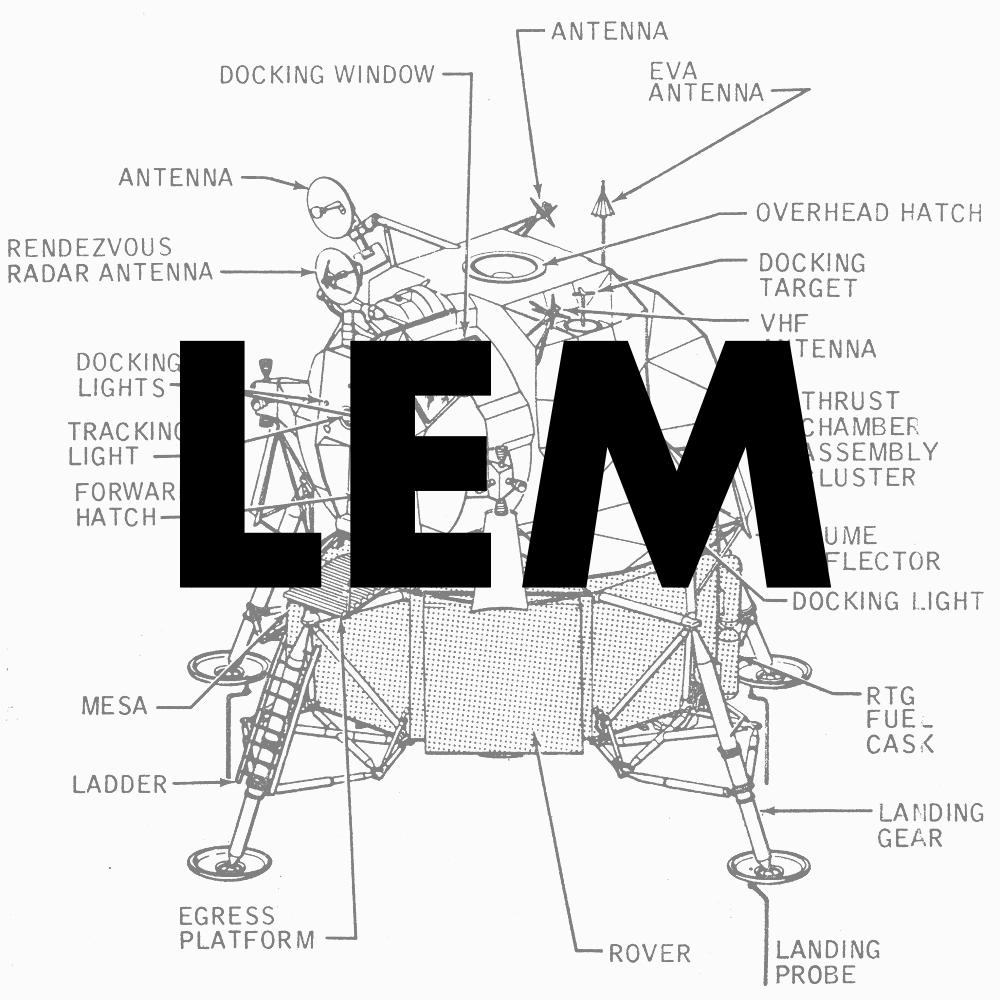
\includegraphics[width=1.25cm]{logo_LEM.png}%
      
\includegraphics[width=1.25cm]{logo_LAST.png}%
      
\includegraphics[width=1.25cm]{logo_Indigo.png}%
      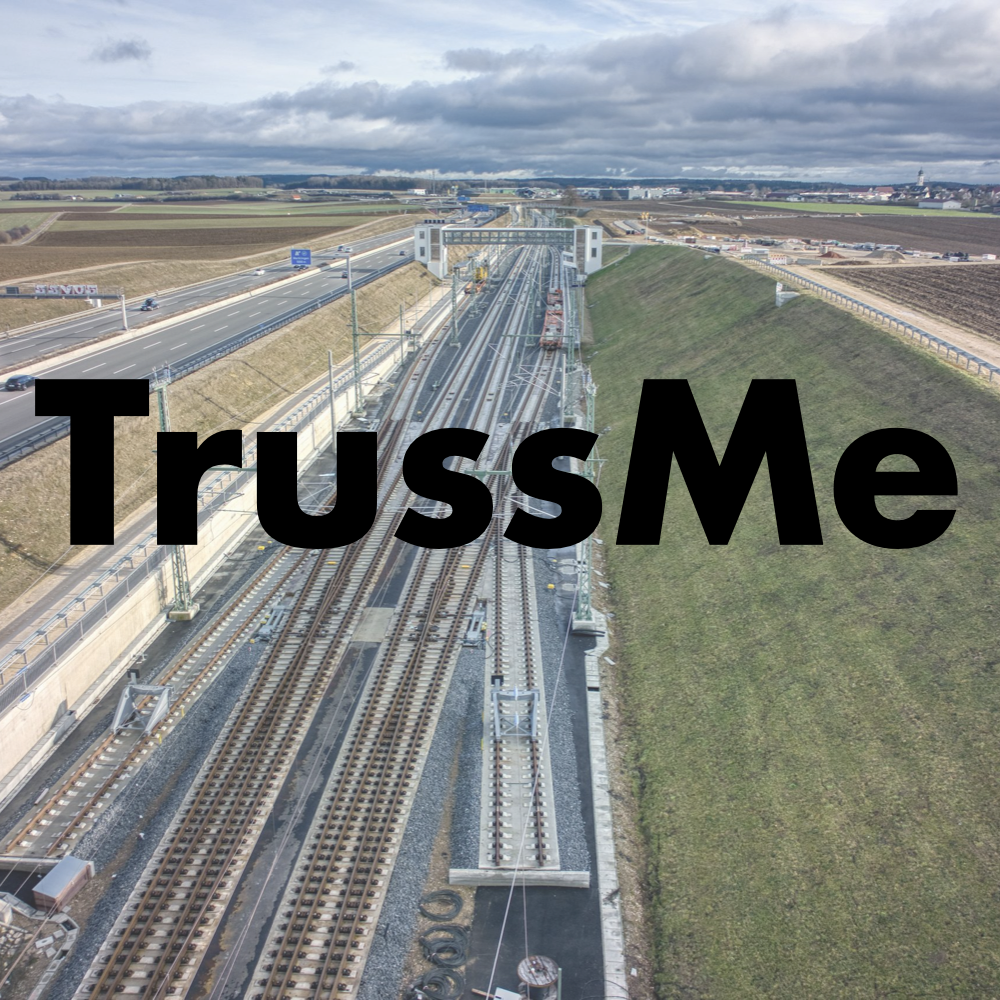
\includegraphics[width=1.25cm]{logo_TrussMe.png}%
      \includegraphics[width=1.25cm]{logo_TrussMe-FEM.png}%
      
\includegraphics[width=1.25cm]{logo_Lime.png}%
      
\includegraphics[width=1.25cm]{logo_LimeRickey.png}
    \end{figure}
  \end{itemize}
\end{frame}

\begin{frame}[plain]{%
  \large%
  Symbolic Computation Methods for the Numerical %
  Solution of Dynamic Systems Described by %
  Differential-Algebraic Equations
  }{Davide Stocco}
  \vfill
  \raggedright{\fontfamily{qag}\selectfont\huge\color{tx_sl_color}\bfseries{Thank you for your attention!}} \\[0.5em]
  \raggedleft{\fontfamily{qag}\selectfont\huge\color{tx_sl_color}\bfseries{Questions?}}
\end{frame}

% That's all Folks!
%!TEX root = main.tex

\begin{frame}{Bibliography}
  \fullcite{stocco2024physical}
  \nocite{stocco2024symbolic}
  \printbibliography[heading=none]
\end{frame}

% That's all Folks!

\end{document}

% That's all Folks!